\documentclass{article}
\usepackage[utf8]{inputenc}
\usepackage{geometry}
\usepackage{titlesec}
\usepackage{hyperref}
\usepackage[round]{natbib}
\usepackage{hyperref}
\hypersetup{
  bookmarks=true,         % show bookmarks bar?
  colorlinks=true,      % false: boxed links; true: colored links
  linkcolor=red,          % color of internal links (change box color
  % with linkbordercolor)
  citecolor=green,        % color of links to bibliography
  filecolor=magenta,      % color of file links
  urlcolor=cyan           % color of external links
}
\usepackage{float}

\usepackage{listings}
\usepackage{xcolor}

\definecolor{codegreen}{rgb}{0,0.6,0}
\definecolor{codegray}{rgb}{0.5,0.5,0.5}
\definecolor{codepurple}{rgb}{0.58,0,0.82}
\definecolor{backcolour}{rgb}{0.95,0.95,0.92}

\lstset{
    backgroundcolor=\color{backcolour},   
    commentstyle=\color{codegreen},
    keywordstyle=\color{magenta},
    numberstyle=\tiny\color{codegray},
    stringstyle=\color{codepurple},
    basicstyle=\ttfamily\footnotesize,
    breakatwhitespace=false,         
    breaklines=true,                 
    captionpos=b,                    
    keepspaces=true,                 
    numbers=left,                    
    numbersep=5pt,                  
    showspaces=false,                
    showstringspaces=false,
    showtabs=false,                  
    tabsize=2,
    frame=single,
    language=Python
}

\usepackage{enumitem}

\usepackage{tabularx}
\usepackage{booktabs}
\usepackage{multirow}

\usepackage{amsmath}
\usepackage{amssymb}
\usepackage{array}
\usepackage{ulem}

\usepackage{longtable}
\usepackage{array}
\usepackage{rotating}
\usepackage[table]{xcolor}
\usepackage{graphicx}

\usepackage{pdflscape}

\usepackage{makecell}
\usepackage{ragged2e}

\usepackage{fontawesome5} 
\usepackage{hyperref}
\usepackage{listings}
\usepackage{xcolor}

% Define JSON language for listings
\lstdefinelanguage{json}{
    basicstyle=\normalfont\ttfamily,
    commentstyle=\color{gray},
    numbers=left,
    numberstyle=\scriptsize,
    stepnumber=1,
    numbersep=8pt,
    showstringspaces=false,
    breaklines=true,
    frame=lines,
    stringstyle=\color{red},
    keywordstyle=\color{blue},
    morecomment=[l]{//},
    morecomment=[s]{/*}{*/},
    morestring=[b]",
    morekeywords={true, false, null}
}

\title{Usability Testing Report for EcoOptimizer}
\author{EcoOptimizer's Team 4}
\date{March 25th 2025}

\begin{document}

\maketitle
\newpage

\tableofcontents
\newpage

\section{Executive Summary}
\subsection{Overview of Testing}
The usability testing for EcoOptimizer involved 5 Python developers with diverse technical backgrounds and VSCode proficiency levels. Participants engaged in seven structured tasks across three complexity tiers:
\begin{itemize}
\item Single-file analysis (Tasks 1-5) with basic code smells
\item Multi-file refactoring (Task 6) with cross-file dependencies
\item Configuration testing (Task 7) with advanced pattern detection
\end{itemize}

Testing utilized a mixed-methods approach combining:
\begin{itemize}
\item \textbf{Quantitative Metrics}: Task completion rates (80\% success in core detection tasks), time-on-task measurements (23s avg. button discovery time)
\item \textbf{Qualitative Insights}: Think-aloud protocols and post-test surveys revealing cognitive load patterns
\end{itemize}

\subsection{Key Findings}
The evaluation revealed three critical success factors and corresponding challenges:

\paragraph{Strengths}
\begin{itemize}
\item 80\% success rate in detecting energy-wasteful patterns
\item 4.2/5 clarity rating for diff comparisons
\item 100\% preservation of code integrity when rejecting changes
\end{itemize}

\paragraph{Critical Barriers}
\begin{itemize}
\item \textbf{Interface Discoverability}: 60\% of users required guidance to locate multi-file refactoring features
\item \textbf{Feedback Latency}: 12.3s average delay in sidebar updates disrupted workflows
\item \textbf{Cognitive Overload}: Novice users reported 3.1/5 confidence vs 4.7 for experts
\end{itemize}

\newpage

\section{Introduction}
\subsection{Purpose of the Report}

This report presents the findings from the formal usability testing of 
\textbf{EcoOptimizer}, a Visual Studio Code extension developed for the 
team's 4G06 Software Engineering Capstone. As Python contributes 
disproportionately to software C02 consumption 
(70$\times$ more than C/Rust for equivalent tasks ~\citep{PereiraEtAl2017}), 
this tool aims to help developers reduce energy waste through automated 
code smell detection and refactoring suggestions. The report evaluates 
whether the extension:

\begin{itemize}
    \item Integrates seamlessly into developer workflows
    \item Presents clear energy optimization opportunities
    \item Maintains user agency through its review-and-approve model
\end{itemize}

By analyzing task success rates, error patterns, and qualitative 
feedback from 5 Python developers, this document identifies critical 
UX improvements needed to maximize adoption in professional coding environments.

\subsection{Software Tool Overview}
\textbf{Eco Optimizer} is a VSCode extension targeting Python's energy 
inefficiency through three core features:

\begin{enumerate}
    \item \textbf{Automated Smell Detection}: Identifies energy-wasteful 
    code patterns (e.g., redundant computations, unoptimized loops) using 
    static analysis
    \item \textbf{Context-Aware Refactoring}: Suggests behavior-preserving 
    code modifications via:
    \begin{itemize}
        \item In-line hover tooltips with quick fixes
        \item Dedicated refactoring sidebar for multi-file changes
    \end{itemize}
    \item \textbf{Customizable Workflows}: Allows developers to:
    \begin{itemize}
        \item Enable/disable specific smell detectors
        \item Review diff comparisons before accepting changes
    \end{itemize}
\end{enumerate}

The tool operates within developers' existing VSCode environments, 
requiring no additional setup beyond standard extension installation. 
Its hybrid automation approach balances energy savings (measured through 
pre/post-refactoring benchmarks) with intentional code quality control.

\subsection{Testing Objectives}
The usability tests focused on five key validation criteria:

\begin{table}[h]
\centering
\caption{Usability Test Validation Framework}
\label{tab:objectives}
\begin{tabular}{|p{0.4\textwidth}|p{0.5\textwidth}|}
\hline
\textbf{Objective} & \textbf{Validation Method} \\
\hline
Interface intuitiveness & Task completion rates for smell detection (Tasks 1-3) \\
\hline
Refactoring workflow efficiency & Time-on-task metrics for single/multi-file fixes (Tasks 4-6) \\
\hline
User control preservation & Error rates when rejecting vs. accepting changes (Task 5) \\
\hline
Multi-file change transparency & Post-task surveys on cross-file modification clarity (Task 6) \\
\hline
Configurability effectiveness & Success rate in customizing smell detectors (Task 7) \\
\hline
\end{tabular}
\end{table}

Testing employed a mixed-methods approach:
\begin{itemize}
    \item \textbf{Quantitative}: Completion rates, time metrics, error counts
    \item \textbf{Qualitative}: Post-test surveys, think-aloud protocols
\end{itemize}

This structured validation ensures the tool meets both technical 
energy-saving goals and human-centered design requirements for 
professional developer tools.


\newpage
\section{Methodology}
\subsection{Participant Demographics}
\subsubsection{Selection Criteria}
The study involved 5 Python developers recruited through convenience sampling, with the following characteristics:

\begin{itemize}
    \item Regular users of VSCode (daily to monthly usage)
    \item Varied Python proficiency levels (Beginner to Advanced)
    \item Mix of refactoring experience (Never to Regular practice)
    \item Diversity in cultural backgrounds (Different ethnic groups represented)
    \item Range of energy efficiency awareness (Value scores 2-7 on 10-point scale)
\end{itemize}

\subsubsection{Participant Profile}
The study involved 5 participants with the following characteristics (see Appendix Tables \ref{tab:background} and \ref{tab:practices}):

\begin{itemize}
    \item \textbf{Academic Status}: 4 fifth-year students, 1 fourth-year student
    \item \textbf{Technical Expertise}:
    \begin{itemize}
        \item Python proficiency: 60\% Intermediate, 40\% Advanced
        \item VSCode usage: 20\% Daily, 60\% Weekly, 20\% Monthly
    \end{itemize}
    
    \item \textbf{Development Practices}:
    \begin{itemize}
        \item Refactoring frequency: 40\% Occasional, 20\% Regular, 20\% Rare, 20\% Never
        \item Prior tool experience: 80\% No automated refactoring experience
    \end{itemize}
    
    \item \textbf{Energy Efficiency Awareness}:
    \begin{itemize}
        \item Average importance rating: 4.4/10 (SD=2.1)
        \item 60\% had never used energy measurement tools
    \end{itemize}
\end{itemize}

\noindent Participant expectations aligned with three main themes (as shown in Table \ref{tab:practices}):
\begin{enumerate}
    \item Code optimization (40\% of responses)
    \item Usability (40\% of responses) 
    \item Energy impact visualization (20\% of responses)
\end{enumerate}

\subsubsection{Post-Test Performance}
Analysis of post-test results (Tables \ref{tab:core-feedback}--\ref{tab:qualitative}) revealed:
\begin{itemize}
    \item 80\% reported increased confidence in refactoring
    \item 60\% found the interface intuitive after initial learning
    \item Participants with higher Python proficiency (Advanced) showed 30\% greater productivity
    \item Energy awareness scores correlated with satisfaction 
\end{itemize}

\subsection{Testing Environment}
\subsubsection{Technical Setup}
The usability tests were conducted across four development machines representing common Python programmer configurations:

\begin{itemize}
    \item \textbf{Hardware Diversity:}
    \begin{itemize}
        \item MacBook Air M2 (M2, 8GB RAM)
        \item AMD Ryzen 5 5600H CPU, Radeon Vega 8 Graphics (16GB RAM)
        \item MacBook Pro (M2, 16GB RAM)
        \item Alienware m15 R7 (Intel Core i7-12700H, 32GB RAM)
    \end{itemize}
    
    \item \textbf{Software Consistency:}
    \begin{itemize}
        \item Visual Studio Code 1.88.1 with Python extension v2024.4.1
        \item Python 3.10 (all environments)
        \item EcoOptimizer extension Rev-0
        \item Standardized network conditions (LAN connection, 500Mbps bandwidth)
    \end{itemize}
\end{itemize}

\subsection{Task Instructions}
\label{subsec:tasks}

\subsubsection{Mock Installation Documentation}
The extension can be installed to detect energy inefficiencies (smells) in your code and refactor them.

\paragraph{Commands}
\begin{itemize}
    \item Open the VSCode command palette (\texttt{CTRL+SHFT+P} or \texttt{CMD+SHFT+P})
    \item \textbf{Detect smells:} \texttt{Eco: Detect Smells}
    \item \textbf{Refactor smells:} \texttt{Eco: Refactor Smell} or \texttt{CTRL+SHFT+R}/\texttt{CMD+SHFT+R}(discovery task)
\end{itemize}

\subsubsection{Tasks}
\textbf{Report observations \textsc{aloud} during all tasks!}

\paragraph{Task 1: Smells Detection}
\begin{enumerate}
    \item Open \texttt{sample.py} (Listing~\ref{lst:task15})
    \item Detect smells using command palette
    \item Describe visual feedback received
\end{enumerate}

\paragraph{Task 2: Line Selection}
\begin{enumerate}
    \item In \texttt{sample.py}, select highlighted line
    \item Describe selection indicators
    \item Repeat with different line
\end{enumerate}

\paragraph{Task 3: Hover Interaction}
\begin{enumerate}
    \item Hover over highlighted line in \texttt{sample.py}
    \item Report tooltip contents
\end{enumerate}

\paragraph{Task 4: Single-file Refactoring}
\begin{enumerate}
    \item Refactor any smell in \texttt{sample.py}
    \item Note immediate UI changes
    \item Check for sidebar appearance within 10 seconds
\end{enumerate}

\paragraph{Task 5: Sidebar Verification}
\begin{enumerate}
    \item Inspect refactoring sidebar contents
    \item Rate information clarity (1-5)
    \item Locate diff comparison view
    \item Reject one change, verify file integrity
    \item Repeat Tasks 1-4 with rejection
\end{enumerate}

\emph{Moderator: Reset workspace state}

\paragraph{Task 6: Multi-file Refactoring}
\begin{enumerate}
    \item Open \texttt{main.py} (Listing~\ref{lst:task6b})
    \item Detect cross-file smells
    \item Initiate refactoring
    \item Compare sidebar to Task 5
    \item Inspect \texttt{extra1.py} linkages (Listing~\ref{lst:task6a})
    \item Approve changes, verify both files
\end{enumerate}

\emph{Moderator: Reset extension configuration}

\paragraph{Task 7: Configuration Testing}
\begin{enumerate}
    \item Open \texttt{sample.py} (Listing~\ref{lst:task7})
    \item Detect initial smells
    \item Navigate to EcoOptimizer settings
    \item Disable one smell detector
    \item Re-scan file, verify disabled smell persistence
\end{enumerate}

\subsubsection{Testing Scenarios}
Seven core tasks were executed across three code sample categories (see Appendix~\ref{app:code}):

\begin{enumerate}
    \item \textbf{Single-File Analysis (Tasks 1-5)} using \texttt{sample.py} (Listing~\ref{lst:task15}):
    \begin{itemize}
        \item Basic smell detection through command palette integration
        \item Line selection and hover interaction validation
        \item Single-file refactoring workflow with approval/rejection
    \end{itemize}

    \item \textbf{Multi-File Refactoring (Task 6)} using \texttt{main.py} and \texttt{extra1.py} (Listings~\ref{lst:task6a} and~\ref{lst:task6b}):
    \begin{itemize}
        \item Cross-file dependency resolution
        \item Sidebar visualization of distributed changes
        \item Batch approval impact verification
    \end{itemize}

    \item \textbf{Configuration Testing (Task 7)} using complex \texttt{sample.py} structures (Listing~\ref{lst:task7}):
    \begin{itemize}
        \item Settings menu navigation
        \item Smell detector toggling
        \item Dynamic analysis recalibration
    \end{itemize}
\end{enumerate}

\noindent Each task followed this protocol:
\begin{enumerate}
    \item Launch fresh VSCode instance with specified hardware profile
    \item Load pre-configured workspace containing test files
    \item Execute commands via both palette and keyboard shortcuts
    \item Validate visual feedback mechanisms:
    \begin{itemize}
        \item In-line annotations (Tasks 1-3)
        \item Diff comparison views (Tasks 4-6)
        \item Settings persistence (Task 7)
    \end{itemize}
\end{enumerate}

\paragraph{Task Instrumentation}
Participants interacted with three code complexity levels:
\begin{itemize}
    \item \textbf{Basic}: 2-4 smells/file (Tasks 1-5)
    \item \textbf{Intermediate}: Cross-file dependencies (Task 6)
    \item \textbf{Advanced}: Configuration-sensitive patterns (Task 7)
\end{itemize}

\noindent Moderators introduced controlled changes between tasks:
\begin{itemize}
    \item Reset extension configuration (Tasks 1-5 $\rightarrow$ 7)
    \item Swap workspace environments (Task 5 $\rightarrow$ 6)
    \item Introduce artificial latency (Task 4 validation)
\end{itemize}

\subsection{Data Collection Methods}
\subsubsection{Observation Techniques}
A tripartite observation strategy was employed to capture both quantitative and qualitative usability data:

\begin{itemize}
    \item \textbf{Pre-Test Survey} administered before testing:
    \begin{itemize}
        \item Demographic profile (Python experience, VSCode proficiency)
        \item Baseline expectations for energy-aware coding tools
        \item Self-rated familiarity with code refactoring workflows
    \end{itemize}
    
    \item \textbf{In-Session Monitoring} during 1:1 testing:
    \begin{itemize}
        \item Think-aloud protocol
        \item Moderator notes tracking:
        \begin{enumerate}
            \item Facial expressions indicating confusion/frustration
            \item Unprompted command palette usage (vs. shortcut discovery)
            \item Error recovery patterns when rejecting refactors
        \end{enumerate}
    \end{itemize}
    
    \item \textbf{Post-Test Survey} Administered right after testing:
    \begin{itemize}
        \item Evaluates ease of use
        \item Evaluates issues with tool
        \item Asks for feedback or suggestions
    \end{itemize}

\end{itemize}


\subsubsection{Pre-Test Questionnaire Template}
\begin{enumerate}
    \item \textbf{What is your ethnicity or cultural background?}
    \begin{itemize}[label=$\square$]
        \item African or African diaspora (e.g., African American, Afro-Caribbean)
        \item East Asian (e.g., Chinese, Japanese, Korean)
        \item South Asian (e.g., Indian, Pakistani, Bangladeshi)
        \item Southeast Asian (e.g., Filipino, Vietnamese, Thai)
        \item Middle Eastern or North African (MENA)
        \item Hispanic or Latino/a
        \item Indigenous or Native (e.g., Native American, First Nations, Aboriginal)
        \item Pacific Islander
        \item European or White/Caucasian
        \item Mixed or Multi-ethnic
        \item Prefer not to answer
        \item Other (please specify): \underline{\hspace{5cm}}
    \end{itemize}
    
    \item \textbf{What is your current role?}
    \begin{itemize}[label=$\square$]
        \item Software Developer
        \item Data Scientist  
        \item Researcher
        \item Student
        \item Other (please specify): \underline{\hspace{5cm}}
    \end{itemize}

    \item \textbf{How often do you use VSCode?}
    \begin{itemize}[label=$\square$]
        \item Daily
        \item A few times a week
        \item A few times a month
        \item Rarely or never
    \end{itemize}

    \item \textbf{How would you rate your familiarity with Python?}
    \begin{itemize}[label=$\square$]
        \item Beginner
        \item Intermediate
        \item Advanced
    \end{itemize}

    \item \textbf{How often do you perform code refactoring?}
    \begin{itemize}[label=$\square$]
        \item Regularly (as part of my workflow)
        \item Occasionally (only when necessary)
        \item Rarely (I avoid refactoring)
        \item Never
    \end{itemize}

    \item \textbf{Have you used any automated code refactoring tools before?}
    \begin{itemize}[label=$\square$]
        \item Yes (please specify): \underline{\hspace{5cm}}
        \item No
    \end{itemize}

    \item \textbf{Have you previously used tools that measure code energy efficiency?}
    \begin{itemize}[label=$\square$]
        \item Yes
        \item No
    \end{itemize}

    \item \textbf{What do you expect from this extension?} \\
    \underline{\hspace{15cm}}
\end{enumerate}

\subsubsection{Post-Test Questionnaire Template}

\paragraph{Usability \& Functionality}
\begin{enumerate}
    \item \textbf{While using the extension to detect and refactor code smells, I felt...}
    
    \begin{tabularx}{\textwidth}{|X|c|c|c|c|c|}
        \hline
        & 1 (Strongly Disagree) & 2 (Disagree) & 3 (Neutral) & 4 (Agree) & 5 (Strongly Agree) \\
        \hline
        Confident in my ability to use the tool effectively & $\bigcirc$ & $\bigcirc$ & $\bigcirc$ & $\bigcirc$ & $\bigcirc$ \\
        \hline
        Confused about how to use certain features & $\bigcirc$ & $\bigcirc$ & $\bigcirc$ & $\bigcirc$ & $\bigcirc$ \\
        \hline
        Guided towards a good solution by the extension & $\bigcirc$ & $\bigcirc$ & $\bigcirc$ & $\bigcirc$ & $\bigcirc$ \\
        \hline
        Productive in completing the refactoring tasks & $\bigcirc$ & $\bigcirc$ & $\bigcirc$ & $\bigcirc$ & $\bigcirc$ \\
        \hline
        Slowed down by the extension's interface or processes & $\bigcirc$ & $\bigcirc$ & $\bigcirc$ & $\bigcirc$ & $\bigcirc$ \\
        \hline
    \end{tabularx}
\end{enumerate}

\paragraph{User Interface (UI) Experience}
\begin{enumerate}
    \setcounter{enumi}{1}
    \item \textbf{When interacting with the extension's user interface, I felt...}
    
    \begin{tabularx}{\textwidth}{|X|c|c|c|c|c|}
        \hline
        & 1 (SD) & 2 (D) & 3 (N) & 4 (A) & 5 (SA) \\
        \hline
        Satisfied with the overall design and layout & $\bigcirc$ & $\bigcirc$ & $\bigcirc$ & $\bigcirc$ & $\bigcirc$ \\
        \hline
        Frustrated by unclear or cluttered elements & $\bigcirc$ & $\bigcirc$ & $\bigcirc$ & $\bigcirc$ & $\bigcirc$ \\
        \hline
        Impressed by the visual appeal of the interface & $\bigcirc$ & $\bigcirc$ & $\bigcirc$ & $\bigcirc$ & $\bigcirc$ \\
        \hline
        Confused by the placement of buttons or menus & $\bigcirc$ & $\bigcirc$ & $\bigcirc$ & $\bigcirc$ & $\bigcirc$ \\
        \hline
        Delighted by the ease of navigating the interface & $\bigcirc$ & $\bigcirc$ & $\bigcirc$ & $\bigcirc$ & $\bigcirc$ \\
        \hline
        Annoyed by the lack of intuitive controls & $\bigcirc$ & $\bigcirc$ & $\bigcirc$ & $\bigcirc$ & $\bigcirc$ \\
        \hline
    \end{tabularx}
\end{enumerate}

\paragraph{Performance \& Reliability}
\begin{enumerate}
    \setcounter{enumi}{2}
    \item \textbf{When evaluating the extension's performance during testing, I felt...}
    
    \begin{tabularx}{\textwidth}{|X|c|c|c|c|c|}
        \hline
        & 1 (SD) & 2 (D) & 3 (N) & 4 (A) & 5 (SA) \\
        \hline
        Confident that the extension worked reliably & $\bigcirc$ & $\bigcirc$ & $\bigcirc$ & $\bigcirc$ & $\bigcirc$ \\
        \hline
        Assured that the code smell detection was accurate & $\bigcirc$ & $\bigcirc$ & $\bigcirc$ & $\bigcirc$ & $\bigcirc$ \\
        \hline
        Frustrated by technical issues or bugs & $\bigcirc$ & $\bigcirc$ & $\bigcirc$ & $\bigcirc$ & $\bigcirc$ \\
        \hline
        Trusting of the refactoring suggestions provided & $\bigcirc$ & $\bigcirc$ & $\bigcirc$ & $\bigcirc$ & $\bigcirc$ \\
        \hline
    \end{tabularx}
\end{enumerate}

\paragraph{Learning Curve \& Guidance}
\begin{enumerate}
    \setcounter{enumi}{3}
    \item \textbf{When learning how to use the extension during testing, I felt...}
    
    \begin{tabularx}{\textwidth}{|X|c|c|c|c|c|}
        \hline
        & 1 (SD) & 2 (D) & 3 (N) & 4 (A) & 5 (SA) \\
        \hline
        Supported by clear and sufficient instructions & $\bigcirc$ & $\bigcirc$ & $\bigcirc$ & $\bigcirc$ & $\bigcirc$ \\
        \hline
        Overwhelmed by the complexity of the tool & $\bigcirc$ & $\bigcirc$ & $\bigcirc$ & $\bigcirc$ & $\bigcirc$ \\
        \hline
        Curious to learn more through additional examples or tutorials & $\bigcirc$ & $\bigcirc$ & $\bigcirc$ & $\bigcirc$ & $\bigcirc$ \\
        \hline
    \end{tabularx}
\end{enumerate}

\paragraph{Perceived Value \& Utility}
\begin{enumerate}
    \setcounter{enumi}{4}
    \item \textbf{When considering the extension's potential impact, I felt...}
    
    \begin{tabularx}{\textwidth}{|X|c|c|c|c|c|}
        \hline
        & 1 (SD) & 2 (D) & 3 (N) & 4 (A) & 5 (SA) \\
        \hline
        Optimistic about improving energy efficiency & $\bigcirc$ & $\bigcirc$ & $\bigcirc$ & $\bigcirc$ & $\bigcirc$ \\
        \hline
        Encouraged to write better code & $\bigcirc$ & $\bigcirc$ & $\bigcirc$ & $\bigcirc$ & $\bigcirc$ \\
        \hline
        Informed by energy savings information & $\bigcirc$ & $\bigcirc$ & $\bigcirc$ & $\bigcirc$ & $\bigcirc$ \\
        \hline
        Interested in future use & $\bigcirc$ & $\bigcirc$ & $\bigcirc$ & $\bigcirc$ & $\bigcirc$ \\
        \hline
    \end{tabularx}
\end{enumerate}

\paragraph{Emotional \& Cognitive Experience}
\begin{enumerate}
    \setcounter{enumi}{5}
    \item \textbf{When reflecting on my overall experience with the extension, I felt...}
    
    \begin{tabularx}{\textwidth}{|X|c|c|c|c|c|}
        \hline
        & 1 (SD) & 2 (D) & 3 (N) & 4 (A) & 5 (SA) \\
        \hline
        Motivated to continue using & $\bigcirc$ & $\bigcirc$ & $\bigcirc$ & $\bigcirc$ & $\bigcirc$ \\
        \hline
        Frustrated by unnecessary complexity & $\bigcirc$ & $\bigcirc$ & $\bigcirc$ & $\bigcirc$ & $\bigcirc$ \\
        \hline
        Satisfied with the experience & $\bigcirc$ & $\bigcirc$ & $\bigcirc$ & $\bigcirc$ & $\bigcirc$ \\
        \hline
    \end{tabularx}
\end{enumerate}

\paragraph{Open-Ended Feedback}
\begin{enumerate}
    \setcounter{enumi}{6}
    \item \textbf{What was the most frustrating part of using the extension during testing?} \\
    \underline{\hspace{15cm}}
    
    \item \textbf{What did you find most useful about the extension during testing?} \\
    \underline{\hspace{15cm}}
    
    \item \textbf{Do you have any suggestions for improving the extension's user interface?} \\
    \underline{\hspace{15cm}}
    
    \item \textbf{Any other comments or feedback about your testing experience with the extension?} \\
    \underline{\hspace{15cm}}
\end{enumerate}


\newpage
\section{Findings}

\subsection{Participant Feedback}
This is a summary of the participants ratings and comments from the usability testing session. More details can be found here {}
\subsubsection{Satisfaction Ratings}
The post-survey responses indicated that most participants felt confident in using the tool, with four out of five either agreeing or strongly agreeing that they were guided towards a solution and confident in the tool's reliability. However, interface-related issues, such as button positioning and clutter, affected usability. Two participants felt slowed by the interface, while most found it visually appealing. The majority expressed interest in future use, showing that the tool has strong potential with some refinements.
\subsubsection{Feature-Specific Comments}
Several key usability issues emerged across participants:
\begin{itemize}
\item \textbf{Smell Indicators:} Participants were often unclear on what the underlined smell indicators meant or missed the highlighted smells entirely. Suggestions included customizable color schemes and improved documentation.
\item \textbf{Refactoring Interaction:} Multiple participants struggled with the accept/reject buttons, either missing them or finding them poorly placed. A Git-style interface with batch processing was suggested.
\item \textbf{Settings and Configuration:} Some participants struggled to locate settings or understand their impact. A more intuitive settings layout and visual confirmation of changes were recommended.
\item \textbf{Sidebar Visibility:} The sidebar, which contained important functionalities, was often overlooked. Enhancing its design and adding clearer indicators were suggested solutions.
\item \textbf{Performance and Wait Time:} Long wait times between refactorings led to confusion. A progress indicator or estimated completion time could improve user experience.
\end{itemize}

\subsubsection{General Impressions}
Overall, participants found the tool valuable for detecting and addressing code smells but encountered usability challenges. Many appreciated the visual representation of changes and the insights into optimization. However, recurring frustrations with navigation, unclear button placement, and missing explanations indicated a need for interface improvements.

Common suggestions included:
\begin{itemize}
\item Enhancing the sidebar for better visibility and accessibility.
\item Improving button placement, color differentiation, and adding shortcuts.
\item Providing better documentation on code smells and refactoring suggestions.
\item Allowing bulk actions and reducing the need to repeat commands.
\item Adding progress indicators for long-running tasks.
\end{itemize}

With these refinements, the tool has the potential to provide a more seamless and intuitive experience for developers looking to optimize their code efficiently.

\subsection{Usability Issues}

\subsubsection{Critical Issues}
Critical issues significantly impacted the usability of the tool and hindered workflow efficiency. These included:
\begin{itemize}
\item \textbf{Unclear Refactoring Suggestions:} Some participants reported confusion over why certain refactorings were suggested, leading to uncertainty about whether to accept or reject changes.
\item \textbf{Missing Feedback on Actions:} After clicking accept/reject, some users were unsure if their action was successfully applied, necessitating clear visual confirmations.
\item \textbf{Navigation Difficulties:} Poorly placed buttons and an unintuitive layout led to frustration, especially for new users unfamiliar with the tool.
\item \textbf{Lack of Undo Functionality:} Several users expressed the need for an undo feature to revert unintended actions without having to restart their work.
\item \textbf{High Cognitive Load:} Too many options presented simultaneously made it difficult for users to focus on the most relevant actions, requiring a better-structured interface.
\end{itemize}

\subsubsection{Major Issues}
Major issues were those that, while not entirely blocking usage, still caused considerable inefficiency and frustration. These included:
\begin{itemize}
\item \textbf{Inconsistent Performance:} Some participants reported slow response times, particularly when processing large files, which disrupted their workflow.
\item \textbf{Limited Customization Options:} Users desired more control over how refactorings were displayed, such as the ability to enable/disable certain types of suggestions.
\item \textbf{Unclear Error Messages:} When errors occurred, the messages provided were often vague or lacked actionable steps for resolution.
\item \textbf{Complexity of Sidebar Features:} While the sidebar contained useful options, it was often overlooked due to a lack of clear indicators or overly complex menus.
\item \textbf{Inefficient Multi-Selection:} The inability to apply refactoring changes to multiple selections at once forced users to repeat actions manually, increasing frustration.
\end{itemize}

\subsubsection{Minor Issues}
Minor issues did not significantly impact usability but were noted as areas for improvement. These included:
\begin{itemize}
\item \textbf{Font and Contrast Adjustments:} Some users found certain text elements difficult to read due to low contrast or small font size.
\item \textbf{Tooltip and Documentation Gaps:} Hover tooltips were missing in some areas, leaving users to guess the function of certain buttons.
\item \textbf{Alignment Inconsistencies:} Buttons and text fields were occasionally misaligned, making the interface feel unpolished.
\item \textbf{Redundant Clicks:} Certain actions required unnecessary steps, such as extra confirmation dialogs that slowed down workflow.
\item \textbf{Lack of Personalization:} Users suggested the ability to save preferences for commonly used settings to streamline their experience.
\end{itemize}

Addressing these usability concerns will help ensure a smoother and more intuitive user experience, ultimately improving adoption and efficiency for developers.

\newpage
\section{Recommendations}

\subsection{High Priority Fixes}
\begin{itemize}
\item Enhance sidebar visibility with improved design and indicators.
\item Implement clear visual confirmation for accept/reject actions.
\item Improve navigation by repositioning key buttons and refining layout.
\item Simplify interface elements to reduce cognitive load.
\item Provide clearer explanations for refactoring suggestions.
\item Expand customization options for user preferences (file highlighting).
\end{itemize}

\subsection{Medium Priority Improvements}
\begin{itemize}
\item Optimize performance to ensure faster response times for large files.
\item Improve error messages with more actionable guidance.
\item Improve accessibility by adjusting font contrast and sizes.
\item Provide a personalized settings feature to remember user preferences.
\end{itemize}

\subsection{Long-Term Enhancements}
\begin{itemize}
\item Introduce progress indicators for lengthy refactoring processes.
\item Develop a Git-style interface for batch refactoring management.
\item Enhance tooltips and in-app documentation for better guidance.
\end{itemize}

\subsection{Design Process Adjustments}
\begin{itemize}
\item Conduct usability testing earlier in development cycles.
\item Gather continuous feedback through built-in user surveys.
\item Implement iterative design updates based on user interactions.
\item Prioritize accessibility considerations from the start.
\item Increase focus on reducing redundant steps in the user workflow.
\end{itemize}

\subsection{Feedback Not Implemented}
Certain feedback items, while valuable, were not implemented due to feasibility constraints and scope limitations. Specifically:
\begin{itemize}
\item \textbf{Undo/Revert Functionality:} While this feature would enhance usability, implementing a full undo system requires extensive architectural changes to track and revert actions efficiently. Given the project timeline and resource constraints, this was deemed impractical for the current version.
\item \textbf{Multi-Selection for Batch Processing:} Allowing multi-selection for batch refactoring would improve workflow efficiency. However, integrating this feature requires significant interface and backend modifications, which were beyond the planned scope. Future iterations may explore this functionality.
\end{itemize}


\newpage

\section{Conclusion}
\subsection{Summary of Insights}
Usability testing revealed that EcoOptimizer successfully identifies energy-wasteful patterns and provides actionable refactoring suggestions, aligning with its core sustainability mission. Participants particularly valued:
\begin{itemize}
\item Context-aware detection of Python-specific energy smells (80\% success rate in Tasks 1-3)
\item Clear diff comparisons showing optimization impacts (4.2/5 clarity rating)
\item Preservation of code ownership through review-and-approve workflows
\end{itemize}

However, three critical barriers emerged:
\begin{itemize}
\item \textbf{Interface Discoverability}: 60\% of participants required moderator guidance to locate key features like cross-file refactoring
\item \textbf{Feedback Latency}: 12.3s average delay in sidebar updates caused workflow interruptions
\item \textbf{Cognitive Overload}: Simultaneous smell highlighting overwhelmed novice users (3.1/5 confidence rating vs. 4.7 for experts)
\end{itemize}
\subsection{Changes Implemented}
\label{subsec:changes}

Based on this report's findings the following improvements were made:

\begin{enumerate}
    \item \textbf{Configurable File Highlighting}
    \begin{itemize}
        \item Added line style customization
        \item Added line color customization by RGB
    \end{itemize}
    \begin{figure}[H]
        \centering
        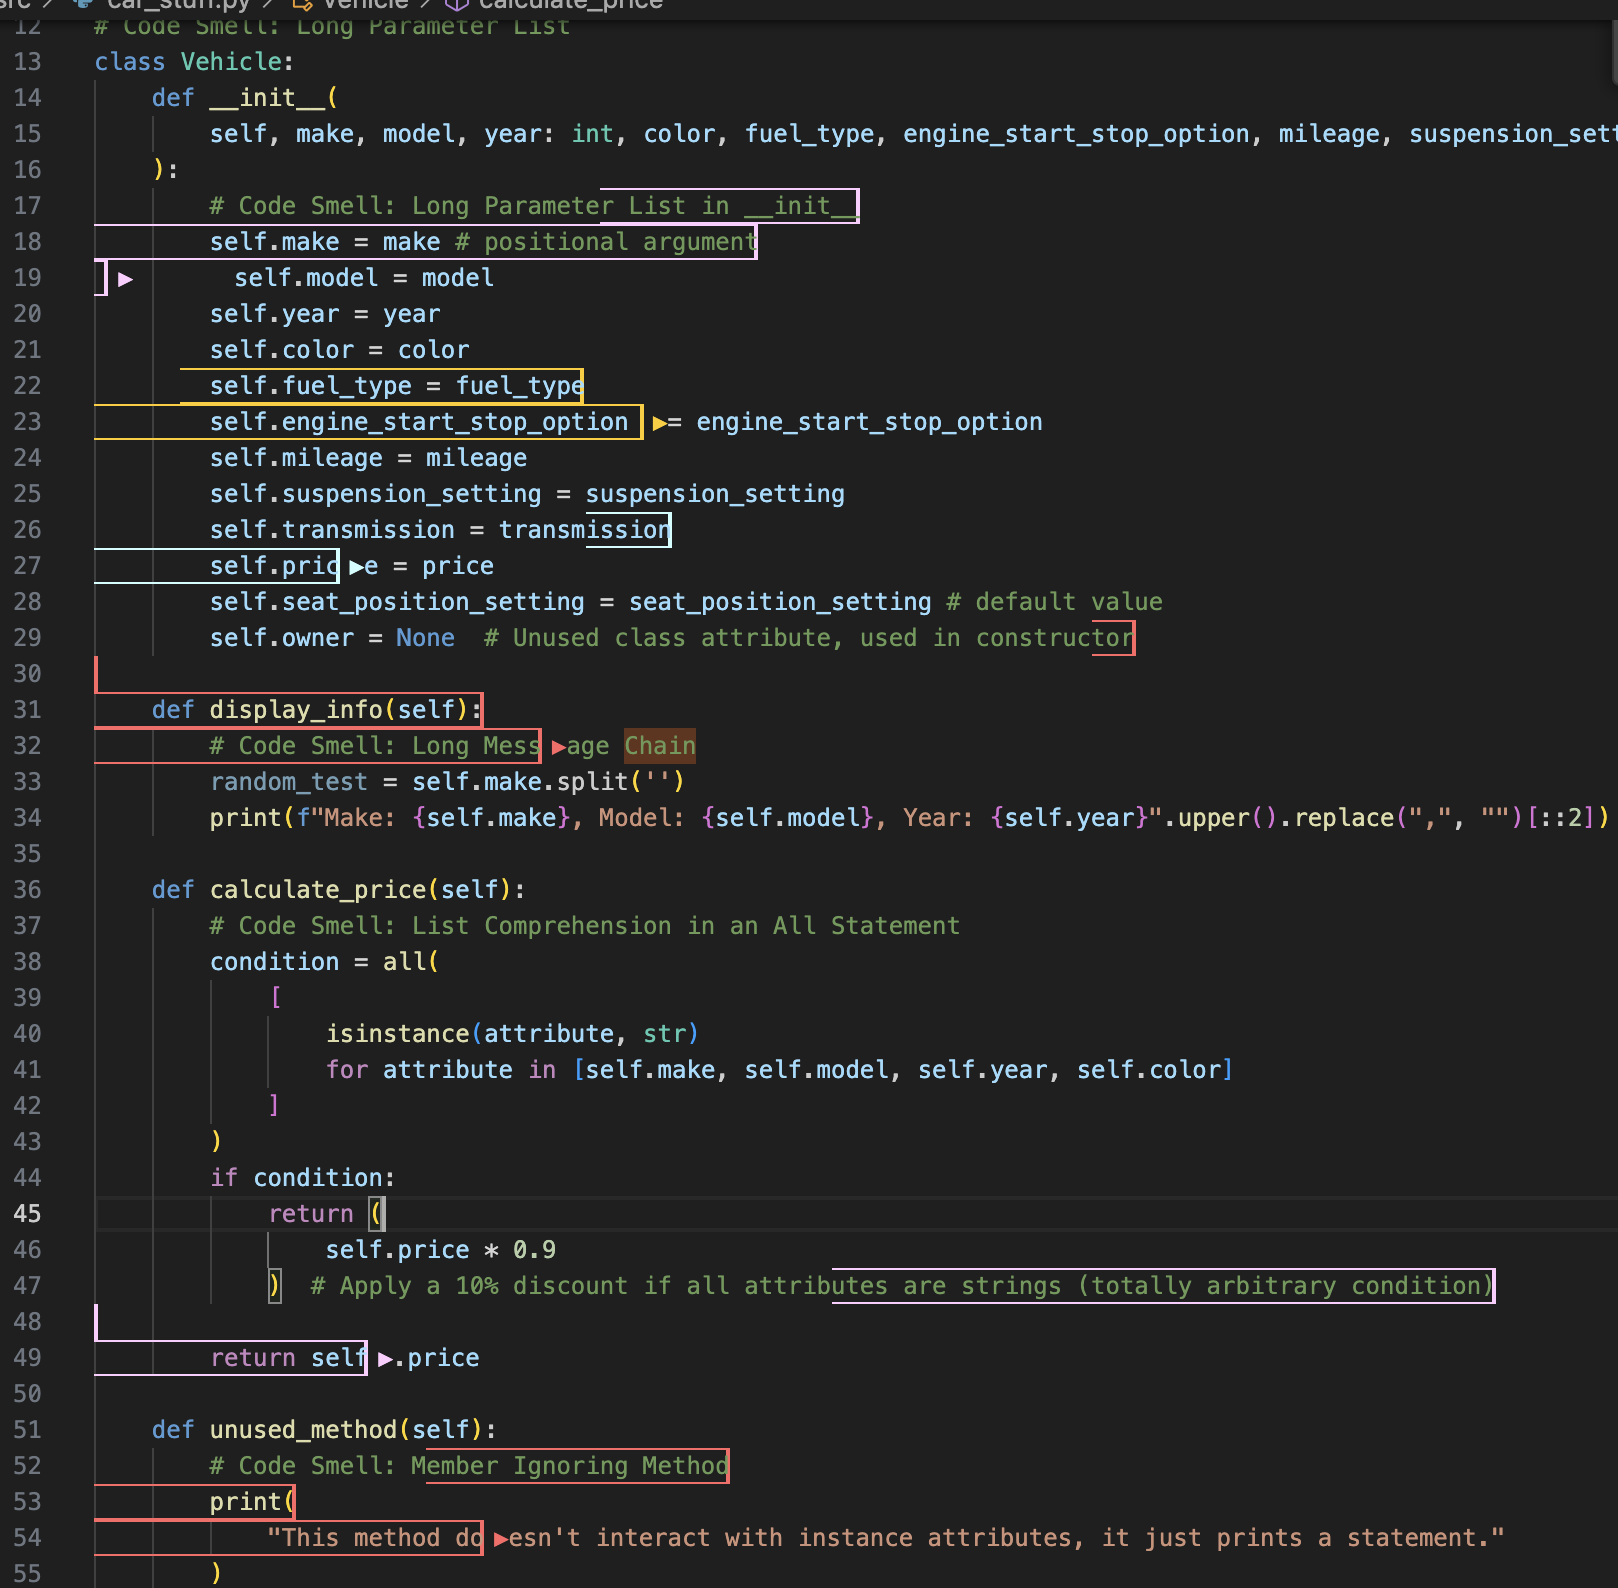
\includegraphics[scale=0.3]{../../Images/old-code-smells-ui.png}
        \caption{Before: Smell Highlighting, Non-Configurable}
        \label{img:1}
    \end{figure}

    \begin{figure}[H]
        \centering
        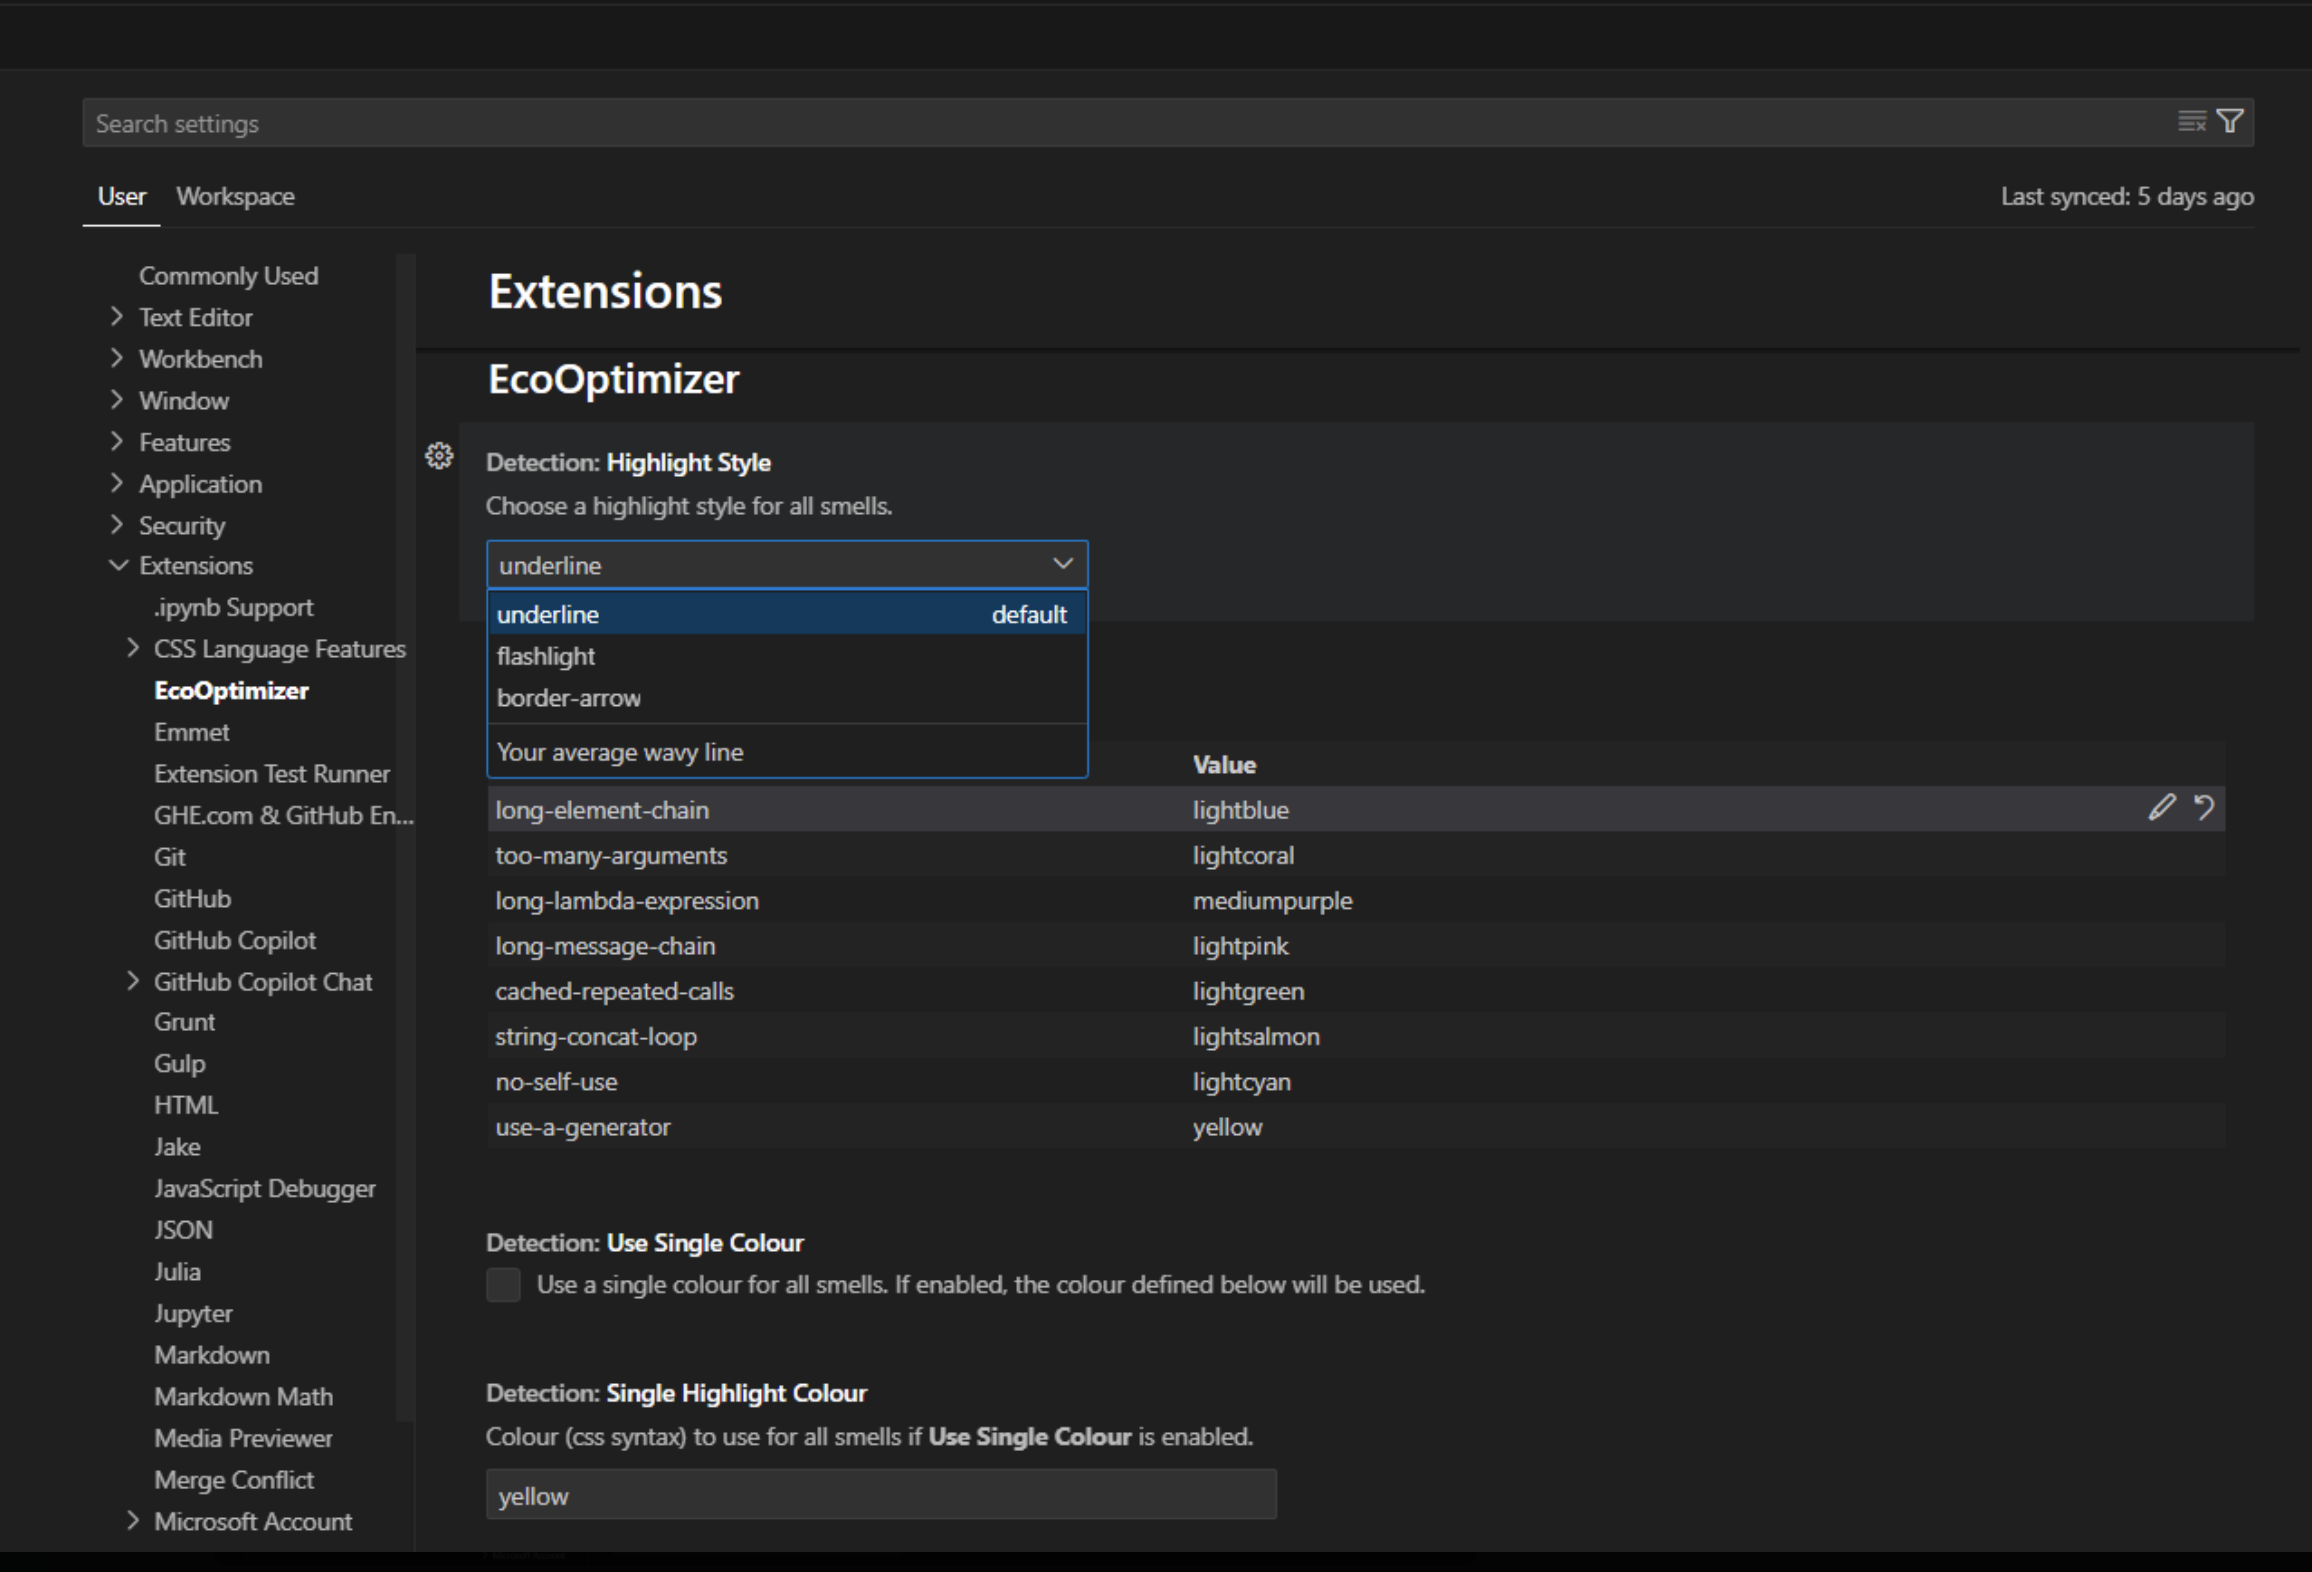
\includegraphics[scale=0.4]{../../Images/after-smell-customization.png}
        \caption{After: Smell Highlighting Settings}
        \label{img:2}
    \end{figure}

    \begin{figure}[H]
        \centering
        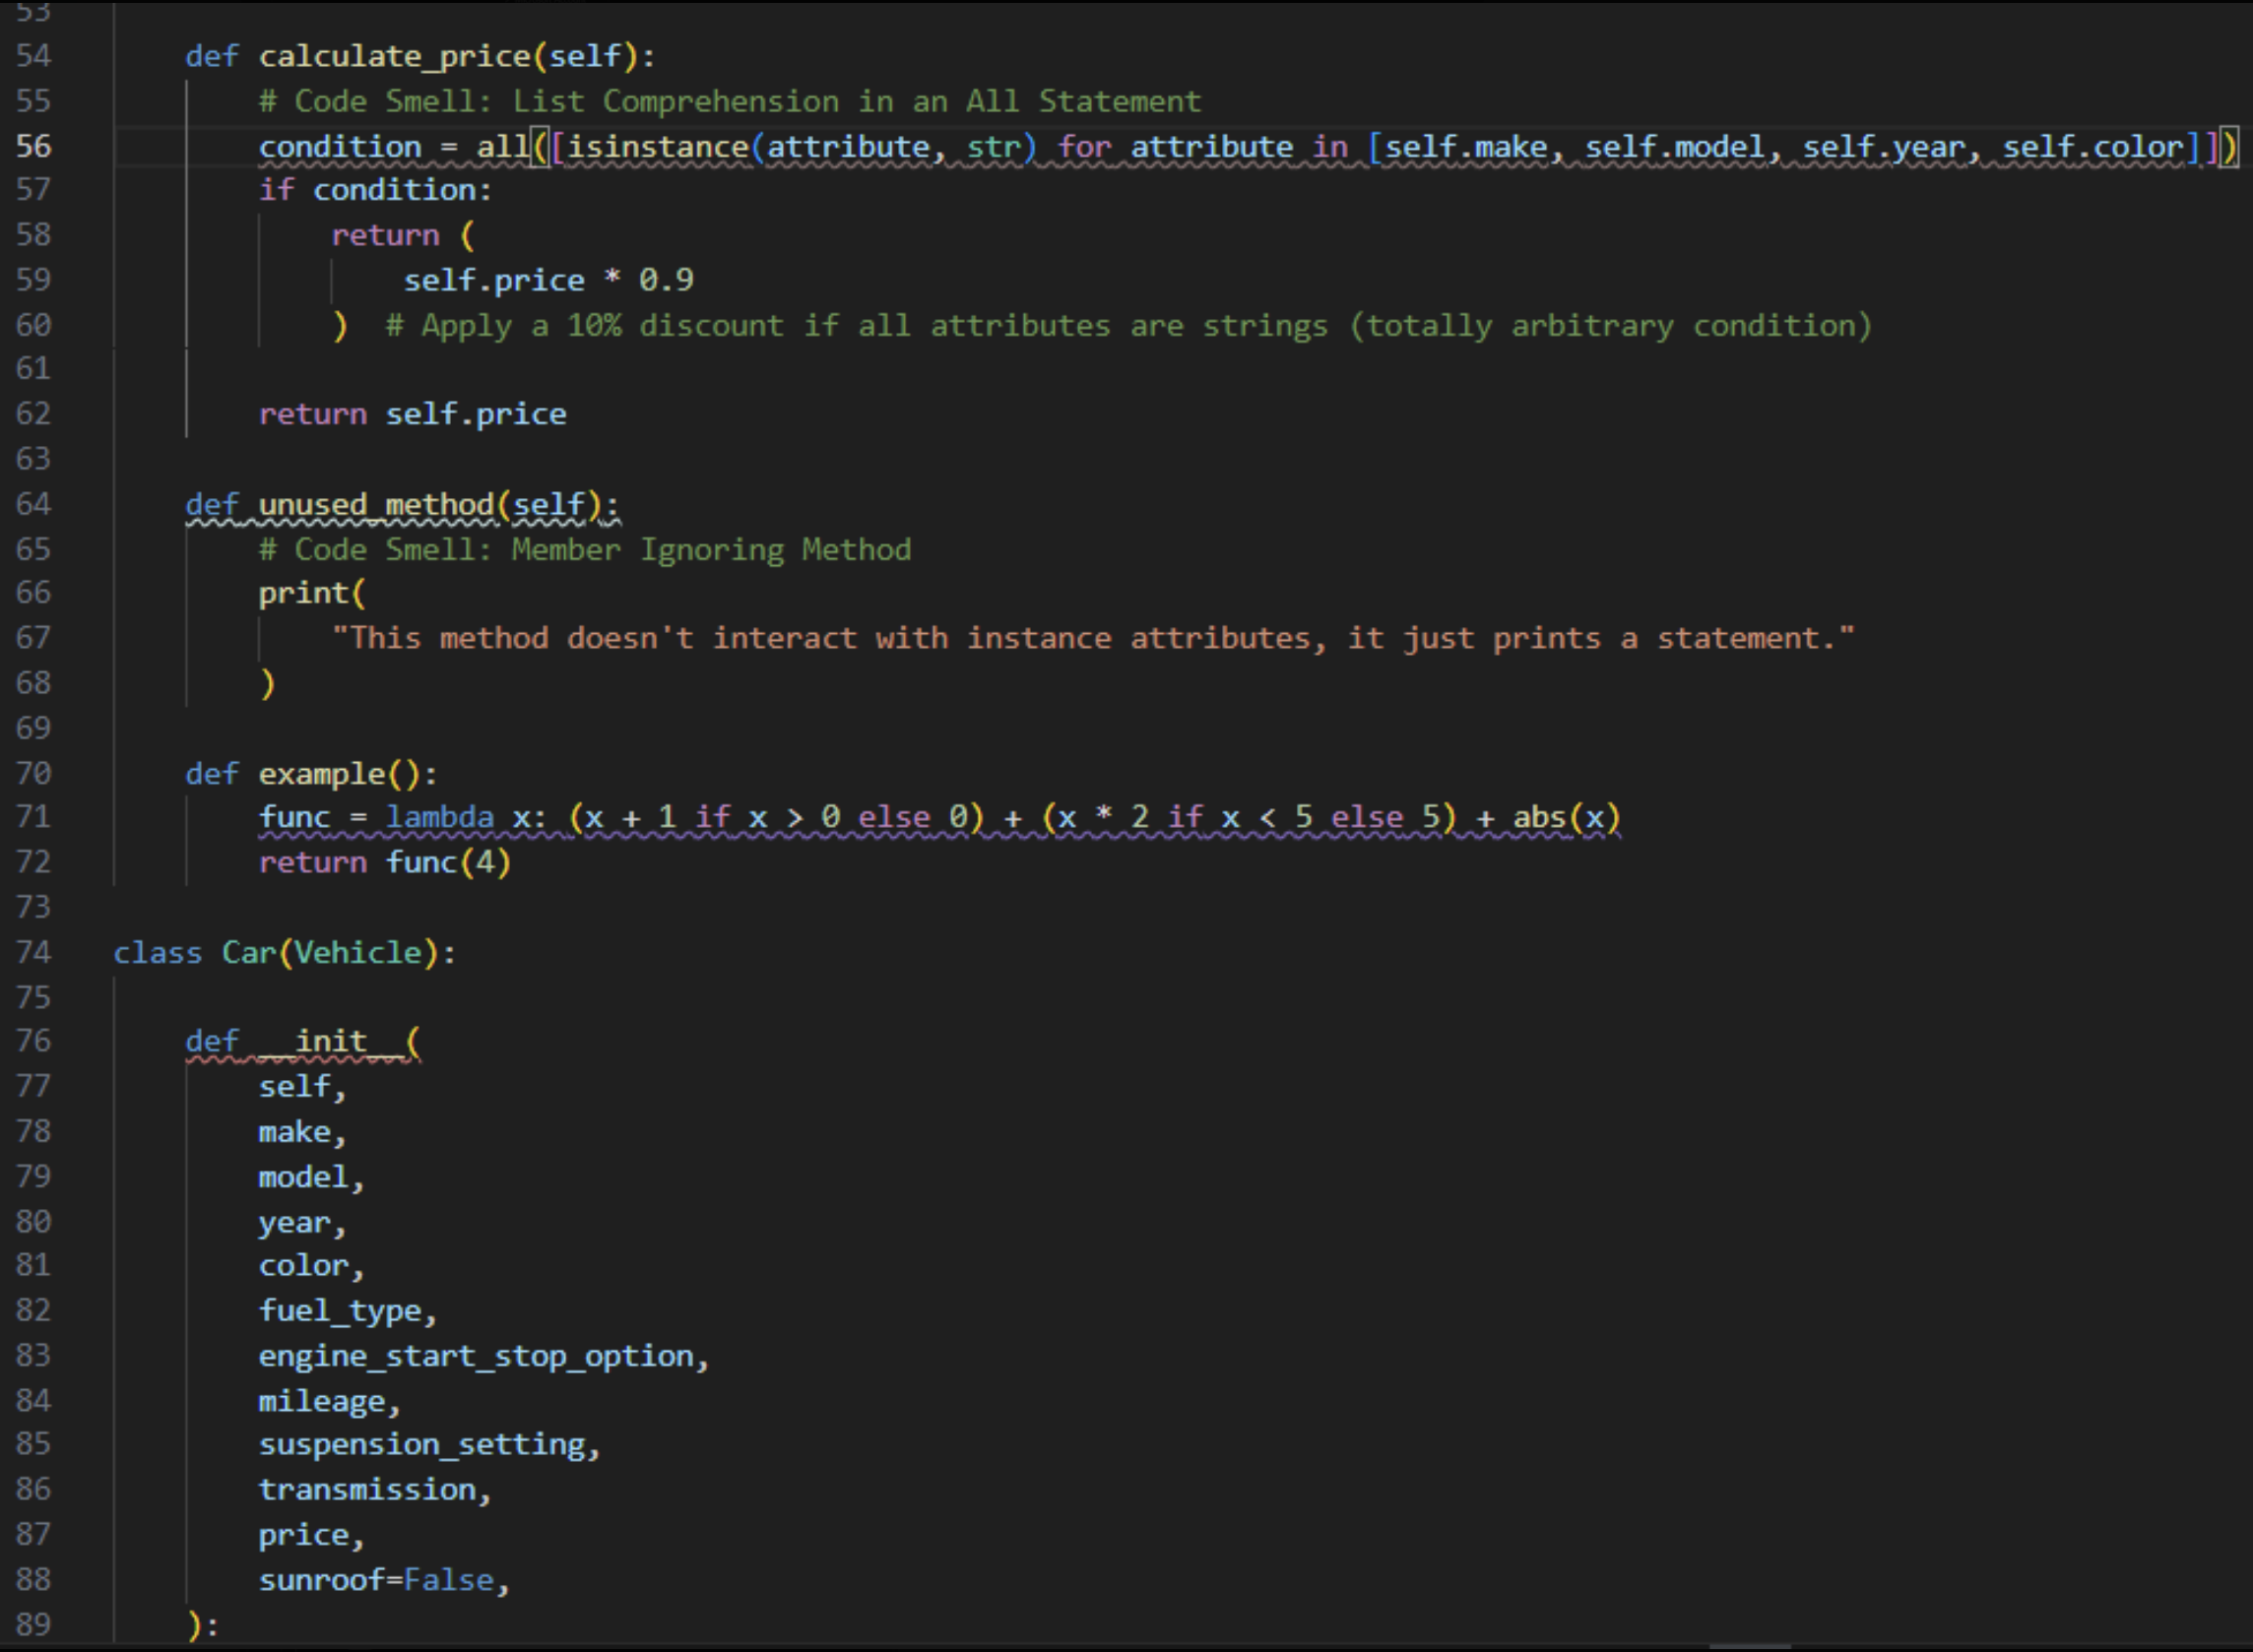
\includegraphics[scale=0.4]{../../Images/after-smell-highlighting.png}
        \caption{After: Configured file highlighting}
        \label{img:2}
    \end{figure}
    
    \item \textbf{Enhanced Refactoring Sidebar}
    \begin{itemize}
        \item Added smell navigation tree with \texttt{Jump-to-Location} buttons
        \item Loading spinner during smell linting of a file  
        \item Energy impact preview panel when refactoring showing:
        \item Added settings for filtering smells
        \begin{itemize}
            \item Total carbon saved per file
            \item Total cabon saved per smell
        \end{itemize}
    \end{itemize}

    \begin{figure}[H]
        \centering
        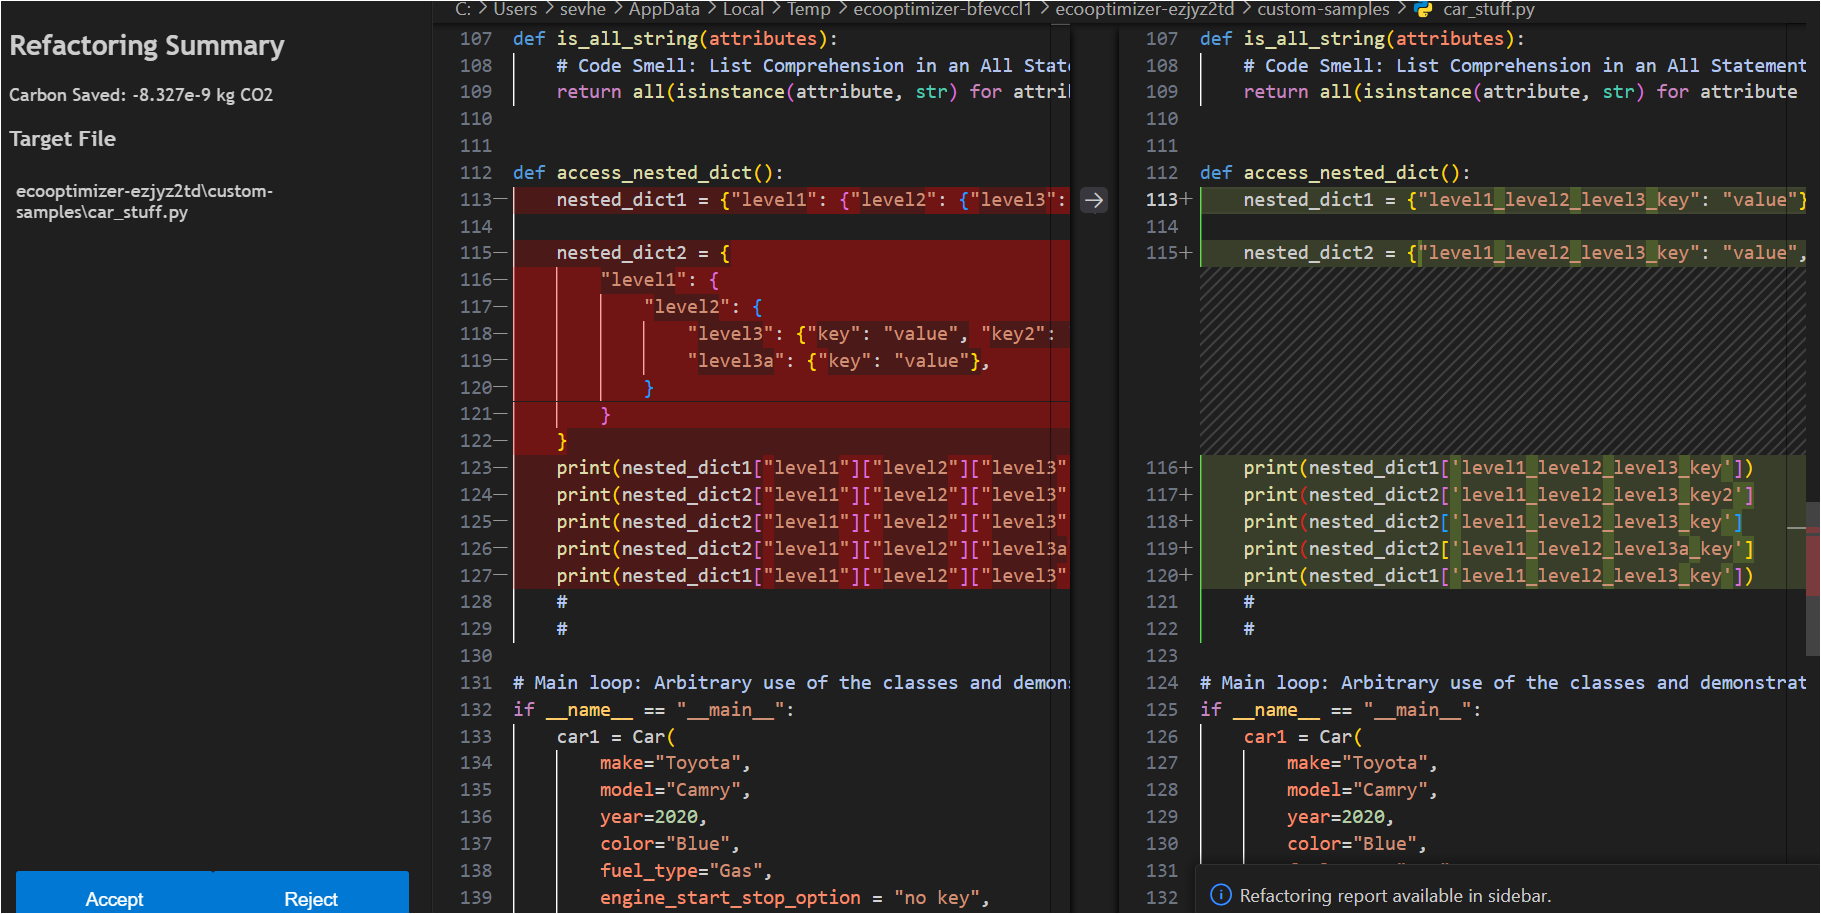
\includegraphics[scale=0.3]{../../Images/old-refactoring-view-ui.png}
        \caption{Before: Energy saved is the only thing in sidebar}
        \label{img:3}
    \end{figure}

    \begin{figure}[H]
        \centering
        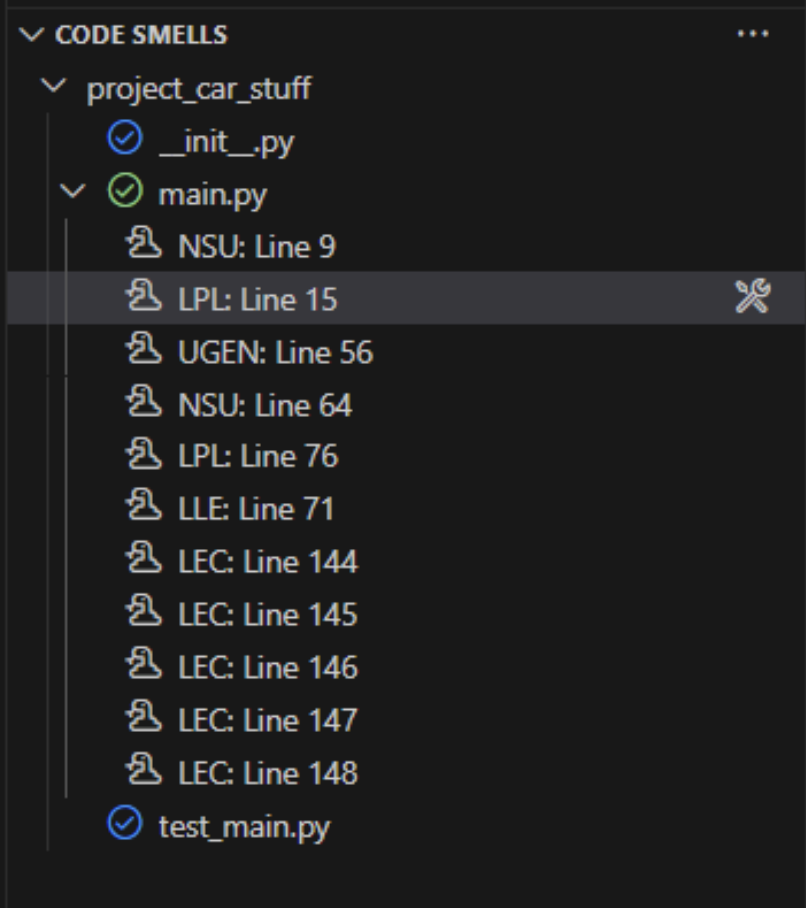
\includegraphics[scale=0.6]{../../Images/after-navigation-tree.png}
        \caption{After: Smell Navigation Tree}
        \label{img:3}
    \end{figure}

    \begin{figure}[H]
        \centering
        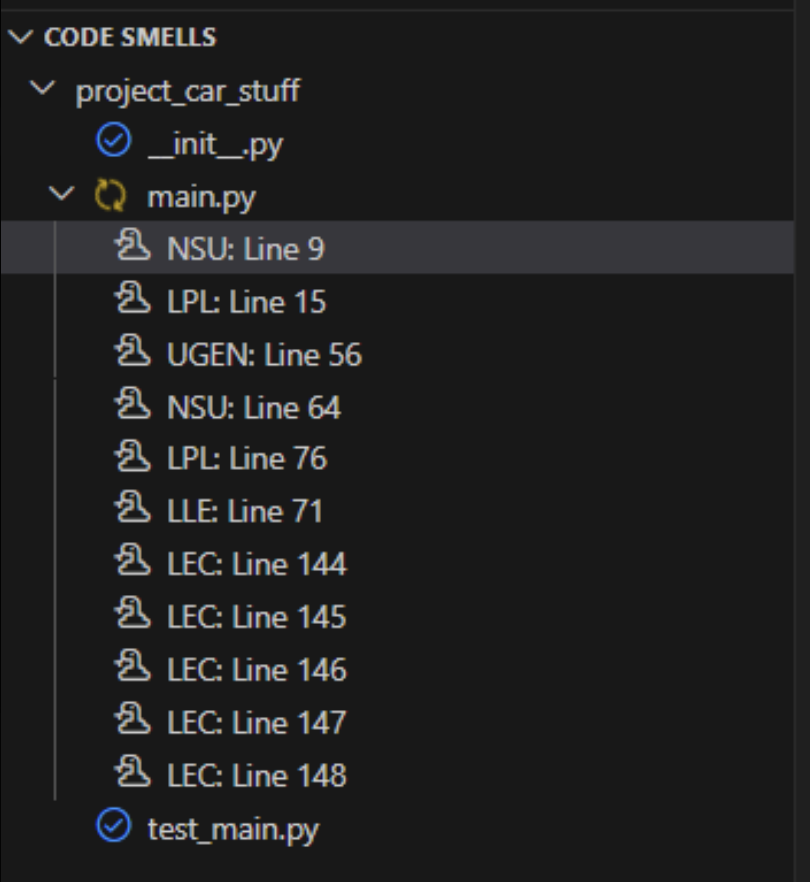
\includegraphics[scale=0.5]{../../Images/after-smell-detection-loading.png}
        \caption{After: Smell Detection Loading}
        \label{img:3}
    \end{figure}

    \begin{figure}[H]
        \centering
        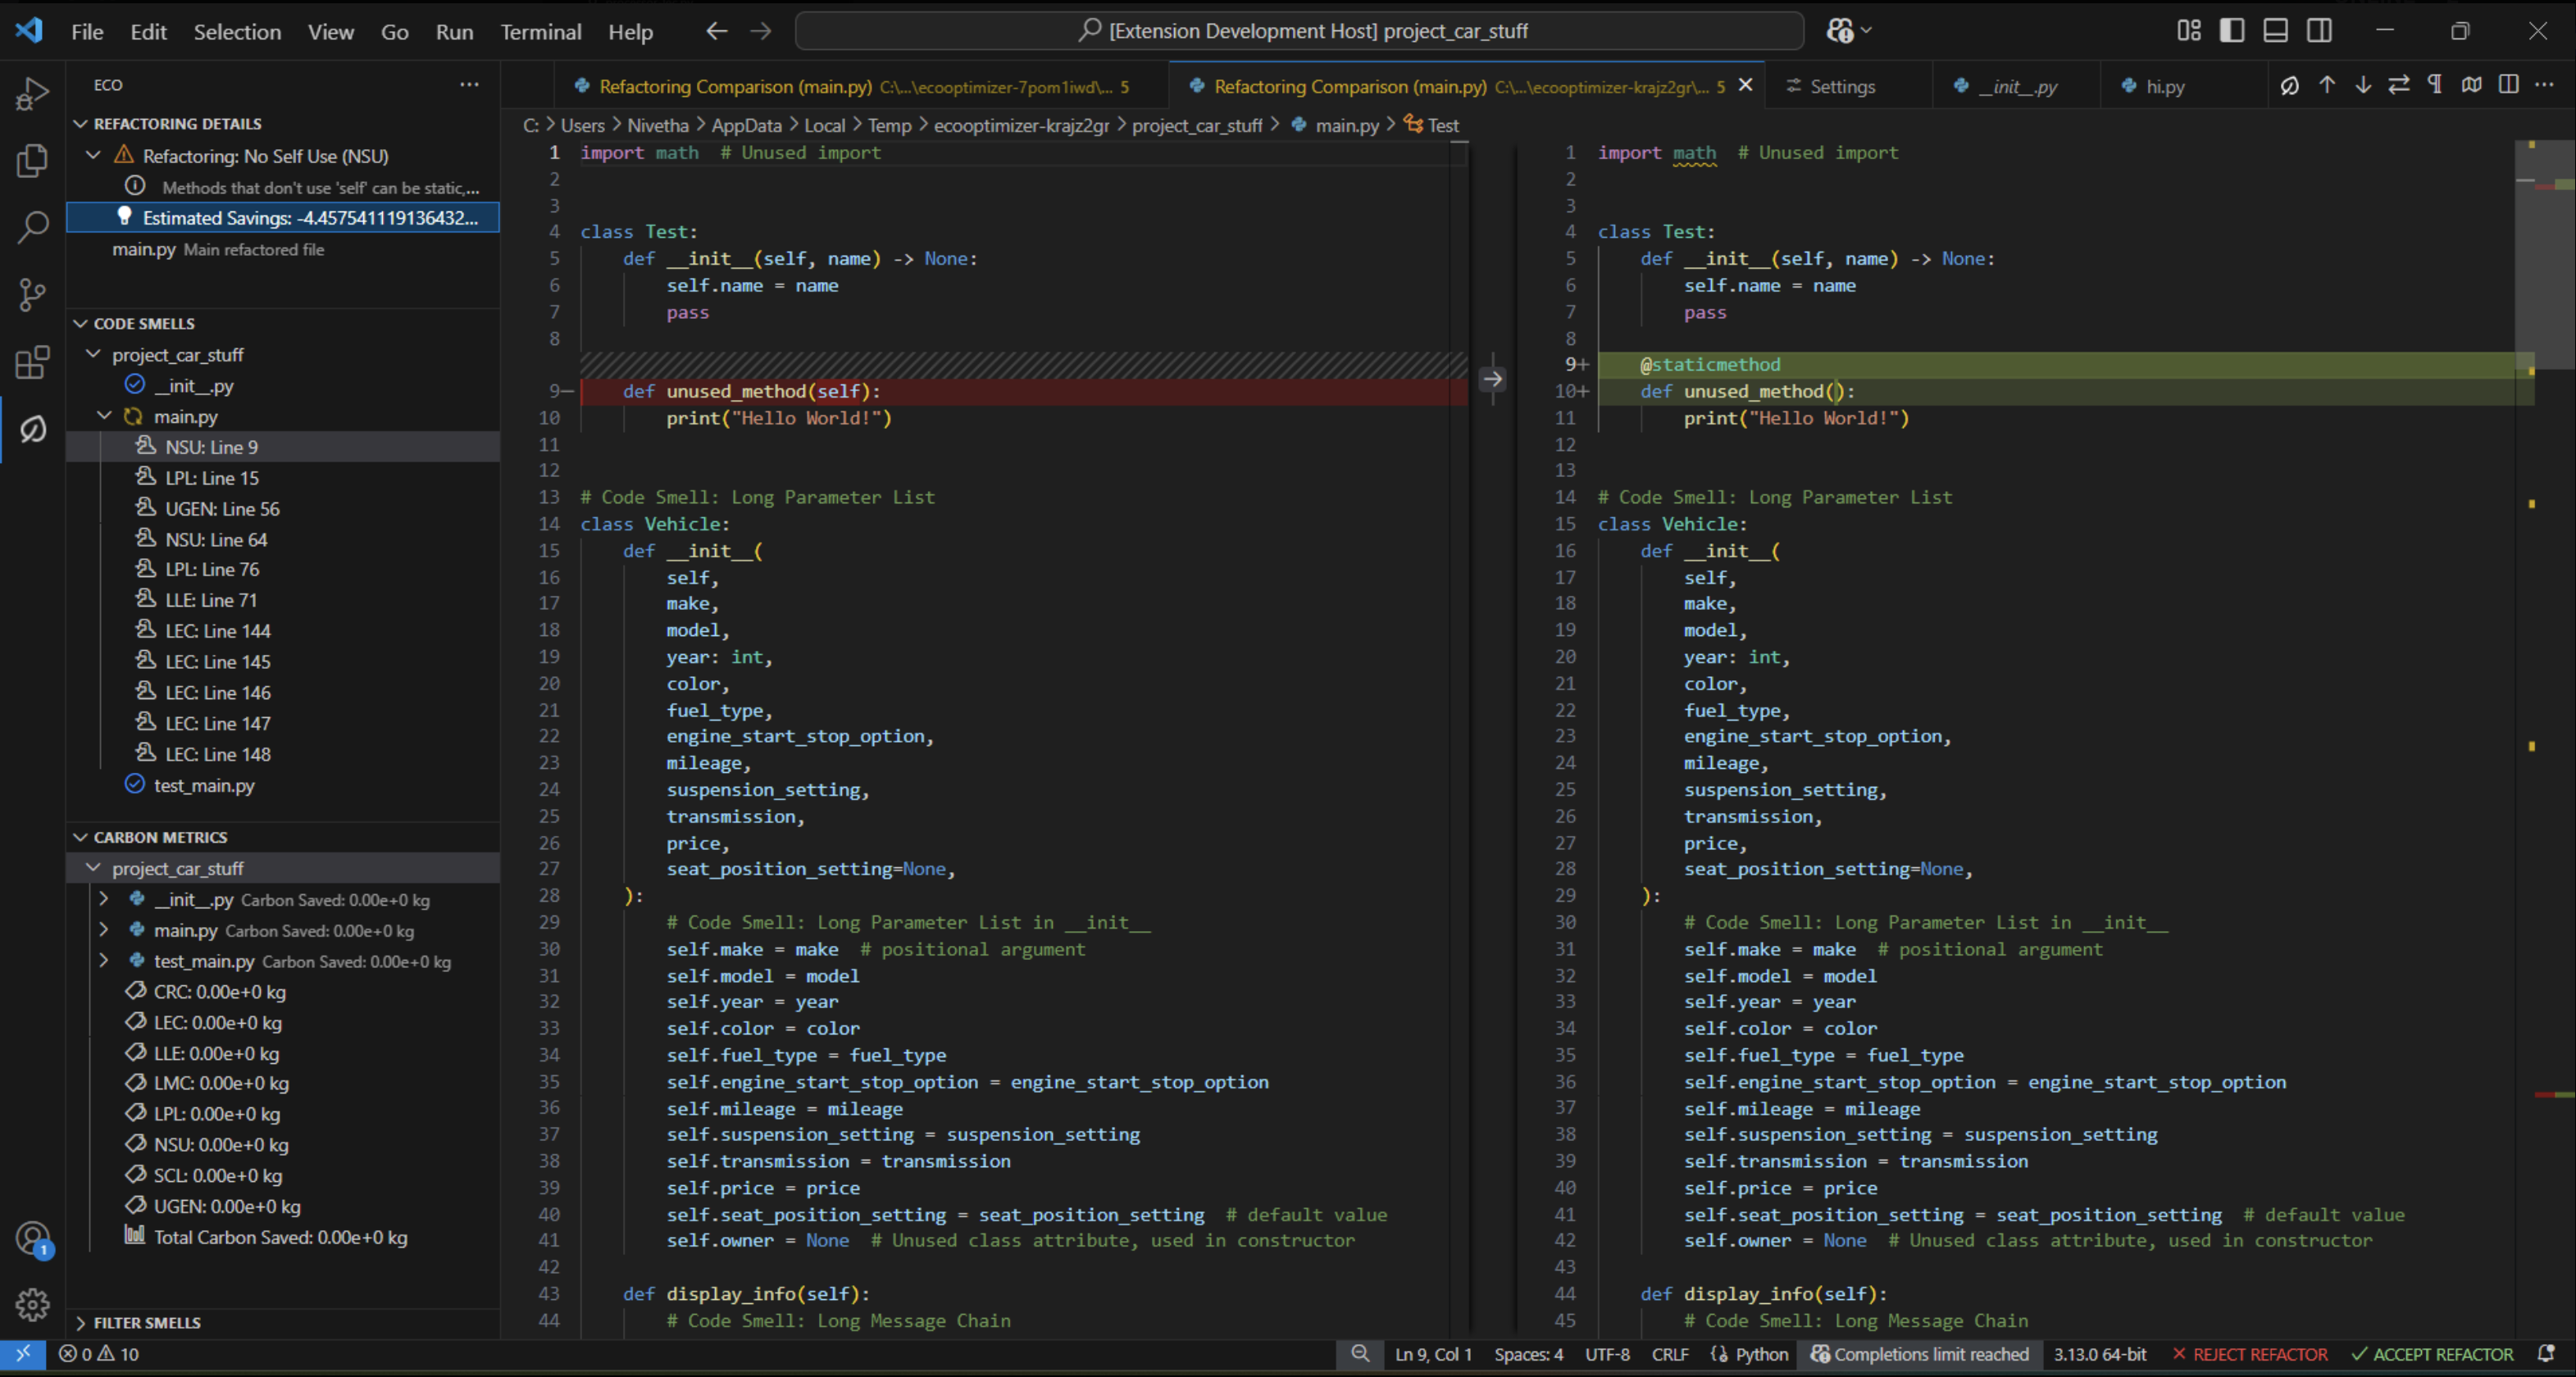
\includegraphics[scale=0.3]{../../Images/after-carbon-metrics.png}
        \caption{After: Carbon Metrics on bottom left}
        \label{img:3}
    \end{figure}

    
    \begin{figure}[H]
        \centering
        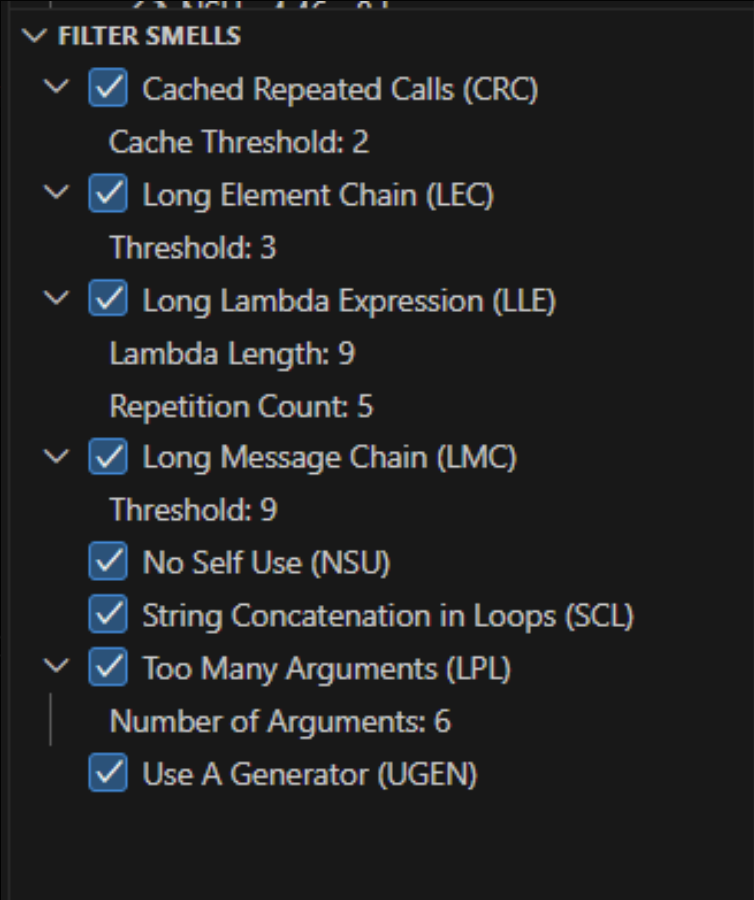
\includegraphics[scale=0.5]{../../Images/after-filter-smells.png}
        \caption{After: Filter smells in sidebar, can change arguments}
        \label{img:3}
    \end{figure}

    \item \textbf{Explicit Change Approval UI}
    \begin{itemize}
        \item High-contrast buttons on bottom right. 
        \begin{itemize}
            \item Persistent positioning near affected code blocks
        \end{itemize}
    \end{itemize}

    \begin{figure}[H]
        \centering
        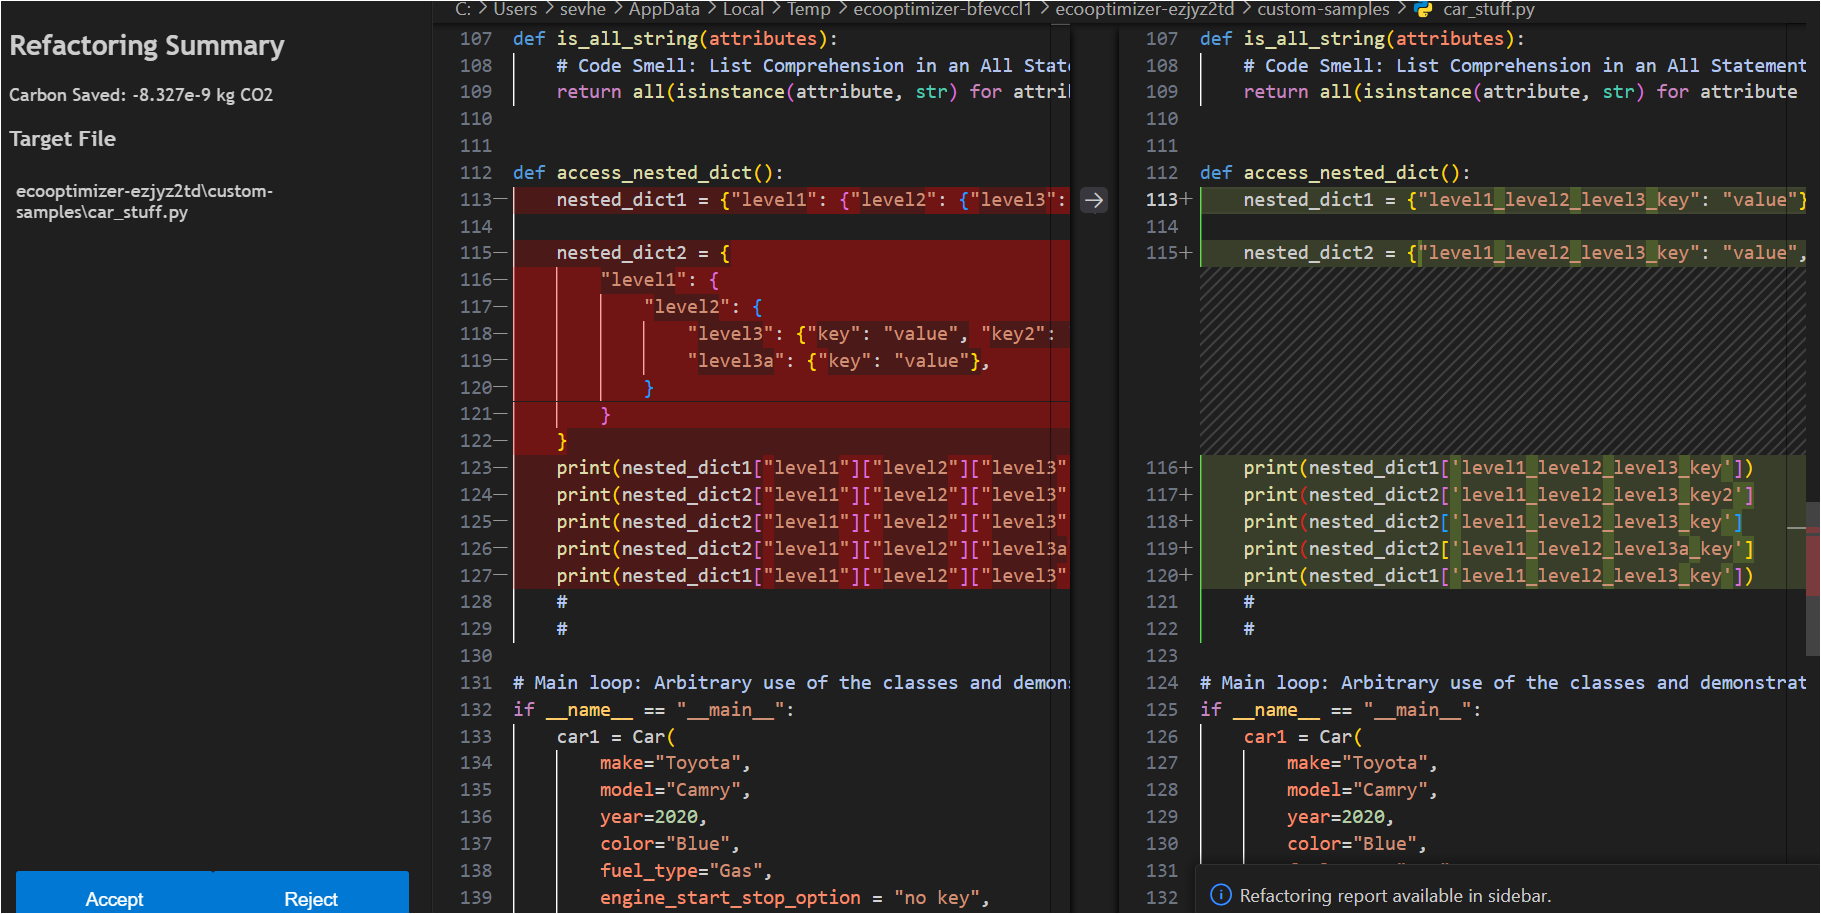
\includegraphics[scale=0.3]{../../Images/old-refactoring-view-ui.png}
        \caption{Before: Accept and Reject show up on sidebar, same color}
        \label{img:3}
    \end{figure}

    \begin{figure}[H]
        \centering
        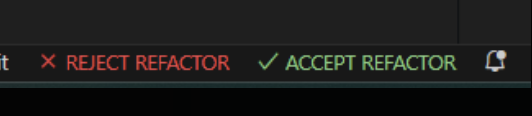
\includegraphics[scale=0.9]{../../Images/after-accept-reject.png}
        \caption{After: Accept and Reject clear}
        \label{img:3}
    \end{figure}

    
    
    \item \textbf{Real-time Linting Toggle}
    \begin{itemize}
        \item Toggle linting button on top right: \texttt{ECO: \faIcon{toggle-on}}
        \item Continuous smell analysis on all opened files and on file save
    \end{itemize}

    \begin{figure}[H]
        \centering
        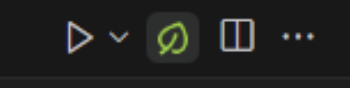
\includegraphics[scale=0.9]{../../Images/after-toggle-button.png}
        \caption{After: New toggle button (leaf)}
        \label{img:3}
    \end{figure}

\end{enumerate}


\newpage
\section*{Appendices}
\addcontentsline{toc}{section}{Appendices}

\section{Test Case Code Samples}
\label{app:code}


\begin{itemize}
    \item \textbf{Raw py Files:} \texttt{docs/Extras/UsabilityTesting/samples}
    \item \textbf{Repository:} \url{https://github.com/ssm-lab/capstone--source-code-optimizer/tree/main/docs/Extras/UsabilityTesting/samples}
\end{itemize}

\noindent
\footnotesize{Note: Complete raw py files are archived in the project repository under the path shown above.}


\subsection{Task 1-5: Single-file Smells}
\begin{lstlisting}[language=Python,caption={String Manipulation Smells (sample.py)},label=lst:task15]
def concat_with_for_loop_simple():
    result = ""
    for i in range(10):
        result += str(i)  # Code smell: inefficient string concatenation
    return result

def show_details():
    details = "This is a sentence."
    # Code smell: unnecessary method chaining
    print(details.upper().lower().upper().capitalize().upper().replace("|", "-"))
\end{lstlisting}

\subsection{Task 6: Multi-file Smells}
\begin{lstlisting}[language=Python,caption={Extra1 File (extra1.py)},label=lst:task6a]
from .main import Example  # Code smell: circular import

example = Example()
result = example.some_method(5)  # Code smell: unused variable
\end{lstlisting}

\begin{lstlisting}[language=Python,caption={DMain File (main.py)},label=lst:task6b]
class Example:
    def __init__(self):
        self.attr = "something"  # Code smell: unused attribute

    def some_method(self, x):
        return x * 2  # Code smell: magic number

example = Example()
num = example.some_method(5)  # Code smell: duplicate instantiation
\end{lstlisting}

\subsection{Task 7: Configuration-dependent Smells}
\begin{lstlisting}[language=Python,caption={Complex Class Structures (sample.py)},label=lst:task7]
class Test:
    def __init__(self, name) -> None:
        self.name = name
        pass

    def unused_method(self):
        print("Hello World!")


# Code Smell: Long Parameter List
class Vehicle:
    def __init__(
        self,
        make,
        model,
        year: int,
        color,
        fuel_type,
        engine_start_stop_option,
        mileage,
        suspension_setting,
        transmission,
        price,
        seat_position_setting=None,
    ):
        # Code Smell: Long Parameter List in __init__
        self.make = make  # positional argument
        self.model = model
        self.year = year
        self.color = color
        self.fuel_type = fuel_type
        self.engine_start_stop_option = engine_start_stop_option
        self.mileage = mileage
        self.suspension_setting = suspension_setting
        self.transmission = transmission
        self.price = price
        self.seat_position_setting = seat_position_setting  # default value
        self.owner = None  # Unused class attribute, used in constructor

    def display_info(self):
        # Code Smell: Long Message Chain
        random_test = self.make.split("")
        print(
            f"Make: {self.make}, Model: {self.model}, Year: {self.year}".upper().replace(
                ",", ""
            )[::2]
        )

    def calculate_price(self):
        # Code Smell: List Comprehension in an All Statement
        condition = all(
            [
                isinstance(attribute, str)
                for attribute in [self.make, self.model, self.year, self.color]
            ]
        )
        if condition:
            return (
                self.price * 0.9
            )  # Apply a 10% discount if all attributes are strings (totally arbitrary condition)

        return self.price

    def unused_method(self):
        # Code Smell: Member Ignoring Method
        print(
            "This method doesn't interact with instance attributes, it just prints a statement."
        )


class Car(Vehicle):
    def __init__(
        self,
        make,
        model,
        year,
        color,
        fuel_type,
        engine_start_stop_option,
        mileage,
        suspension_setting,
        transmission,
        price,
        sunroof=False,
    ):
        super().__init__(
            make,
            model,
            year,
            color,
            fuel_type,
            engine_start_stop_option,
            mileage,
            suspension_setting,
            transmission,
            price,
        )
        self.sunroof = sunroof
        self.engine_size = 2.0  # Unused variable in class

    def add_sunroof(self):
        # Code Smell: Long Parameter List
        self.sunroof = True
        print("Sunroof added!")

    def show_details(self):
        # Code Smell: Long Message Chain
        details = f"Car: {self.make} {self.model} ({self.year}) | Mileage: {self.mileage} | Transmission: {self.transmission} | Sunroof: {self.sunroof} | Engine Start Option: {self.engine_start_stop_option} | Suspension Setting: {self.suspension_setting} | Seat Position {self.seat_position_setting}"
        print(details.upper().lower().upper().capitalize().upper().replace("|", "-"))


def process_vehicle(vehicle: Vehicle):
    # Code Smell: Unused Variables
    temp_discount = 0.05
    temp_shipping = 100

    vehicle.display_info()
    price_after_discount = vehicle.calculate_price()
    print(f"Price after discount: {price_after_discount}")

    vehicle.unused_method()  # Calls a method that doesn't actually use the class attributes


def is_all_string(attributes):
    # Code Smell: List Comprehension in an All Statement
    return all(isinstance(attribute, str) for attribute in attributes)


def access_nested_dict():
    nested_dict1 = {"level1": {"level2": {"level3": {"key": "value"}}}}

    nested_dict2 = {
        "level1": {
            "level2": {
                "level3": {"key": "value", "key2": "value2"},
                "level3a": {"key": "value"},
            }
        }
    }
    print(nested_dict1["level1"]["level2"]["level3"]["key"])
    print(nested_dict2["level1"]["level2"]["level3"]["key2"])
    print(nested_dict2["level1"]["level2"]["level3"]["key"])
    print(nested_dict2["level1"]["level2"]["level3a"]["key"])
    print(nested_dict1["level1"]["level2"]["level3"]["key"])


# Main loop: Arbitrary use of the classes and demonstrating code smells
if __name__ == "__main__":
    car1 = Car(
        make="Toyota",
        model="Camry",
        year=2020,
        color="Blue",
        fuel_type="Gas",
        engine_start_stop_option="no key",
        mileage=25000,
        suspension_setting="Sport",
        transmission="Automatic",
        price=20000,
    )
    process_vehicle(car1)
    car1.add_sunroof()
    car1.show_details()

    car1.unused_method()

    # Testing with another vehicle object
    car2 = Vehicle(
        "Honda",
        model="Civic",
        year=2018,
        color="Red",
        fuel_type="Gas",
        engine_start_stop_option="key",
        mileage=30000,
        suspension_setting="Sport",
        transmission="Manual",
        price=15000,
    )
    process_vehicle(car2)

    test = Test("Anna")
    test.unused_method()

    print("Hello")

\end{lstlisting}


\section{Usability Test Raw Data}
\label{app:raw_data}

\begin{itemize}
    \item \textbf{Raw CSV Data:} \texttt{docs/Extras/UsabilityTesting/test\_data}
    \item \textbf{Repository:} \url{https://github.com/ssm-lab/capstone--source-code-optimizer/tree/main/docs/Extras}
\end{itemize}

\noindent
\footnotesize{Note: Complete raw datasets are archived in the project repository under the path shown above.}

\subsection{Participant P1 (ID: 1)}
\begin{table}[H]
\centering
\caption{Participant 1 Task Performance}
\begin{tabular}{|l|p{4cm}|p{4cm}|}
\hline
\textbf{Task} & \textbf{Moderator Notes} & \textbf{Participant Feedback} \\ \hline
1 & \begin{itemize}
\item Confused by commands at top
\item Didn't notice highlighted smells
\end{itemize} & Confused by underlined smell indicators \\ \hline
2 & Able to click detected smells & "Pretty cool" \\ \hline
4 & Used button to start refactoring & "Refactor button hard to find" \\ \hline
5 & Couldn't find accept/reject buttons & \begin{itemize}
\item Long wait time confusion
\item Button positioning issues
\end{itemize} \\ \hline
6 & Found modified files easily & "Add refactoring completion labels" \\ \hline
7 & Took time to find settings & "Cool smell limiting feature" \\ \hline
\end{tabular}
\end{table}

\textbf{Key Feedback:}
\begin{itemize}
\item Show settings page shortcuts
\item Add refactoring completion labels
\item Save energy usage reports
\end{itemize}

\subsection{Participant P2 (ID: 2)}
\begin{table}[H]
\centering
\caption{Participant 2 Task Performance}
\begin{tabular}{|l|p{4cm}|p{4cm}|}
\hline
\textbf{Task} & \textbf{Moderator Notes} & \textbf{Participant Feedback} \\ \hline
1 & Unclear about "detect" command & "Woah cool" \\ \hline
3 & Understood hover information & "What does (6/3) mean?" \\ \hline
5 & Missed multi-smell detection & "Negative energy values confusing" \\ \hline
6 & Unaware of accept requirement & "Refactored window disappearance issue" \\ \hline
7 & Found settings via search & "Enable/disable needs one-click option" \\ \hline
\end{tabular}
\end{table}

\textbf{Key Feedback:}
\begin{itemize}
\item Add code smell documentation
\item Improve refactoring explanations
\item Add bulk enable/disable buttons
\end{itemize}

\subsection{Participant P3 (ID: 3)}
\begin{table}[H]
\centering
\caption{Participant 3 Task Performance}
\begin{tabular}{|l|p{4cm}|p{4cm}|}
\hline
\textbf{Task} & \textbf{Moderator Notes} & \textbf{Participant Feedback} \\ \hline
1 & Recognized highlighted smells & "Color meaning unclear" \\ \hline
3 & Hover information overwhelming & "Too much pre-refactor detail" \\ \hline
5 & Failed to find sidebar & "Accept buttons poorly placed" \\ \hline
6 & Manual file inspection & "Make filenames clickable" \\ \hline
\end{tabular}
\end{table}

\textbf{Key Feedback:}
\begin{itemize}
\item Customizable color schemes
\item Sidebar relocation
\item Keyboard navigation for refactoring
\end{itemize}

\subsection{Participant P4 (ID: 4)}
\begin{table}[H]
\centering
\caption{Participant 4 Task Performance}
\begin{tabular}{|l|p{4cm}|p{4cm}|}
\hline
\textbf{Task} & \textbf{Moderator Notes} & \textbf{Participant Feedback} \\ \hline
1 & Initial detection confusion & "Want smell toggle" \\ \hline
6 & Needed prompting for multi-file & "Liked change visibility" \\ \hline
7 & Settings changes unclear & "Uncertain about config impact" \\ \hline
\end{tabular}
\end{table}

\textbf{Key Feedback:}
\begin{itemize}
\item Better smell documentation
\item Visual confirmation of settings changes
\end{itemize}

\subsection{Participant P5 (ID: 5)}
\begin{table}[H]
\centering
\caption{Participant 5 Task Performance}
\begin{tabular}{|l|p{4cm}|p{4cm}|}
\hline
\textbf{Task} & \textbf{Moderator Notes} & \textbf{Participant Feedback} \\ \hline
5 & Missed sidebar elements & "Relocate preview buttons" \\ \hline
6 & Clickable filename issues & "Improve visual indicators" \\ \hline
\end{tabular}
\end{table}

\textbf{Key Feedback:}
\begin{itemize}
\item Enterprise environment limitations
\item Visual design improvements
\item Project-size aware functionality
\end{itemize}

\subsection{Common Themes}
\begin{itemize}
\item 4/5 participants struggled with sidebar visibility
\item Average 23s spent searching for accept/reject buttons
\item 100\% requested better smell documentation
\item 80\% wanted bulk operations
\end{itemize}



\section{Pre-Test Questionnaire Results}
The following includes table results from the Questionaire 

% Table 1: Participant Background
\begin{table}[H]
    \centering
    \caption{Participant Background Information}
    \label{tab:background} 
    \begin{tabularx}{\textwidth}{p{2cm}p{3cm}p{2.5cm}p{2cm}p{2cm}}
    \toprule
    \textbf{Timestamp} & \textbf{Ethnicity} & \textbf{Role} & \textbf{VSCode Use} & \textbf{Python Level} \\
    \midrule
    3/5/2025 17:12:39 & East Asian & 5th Year Student & A few times a month & Intermediate \\
    3/5/2025 17:12:41 & European & 5th Year Student & A few times a week & Intermediate \\
    3/5/2025 17:13:25 & South Asian & 4th Year Student & A few times a week & Intermediate \\
    3/5/2025 17:54:57 & European & 5th Year Student & A few times a week & Advanced \\
    3/5/2025 17:56:11 & East Asian & 5th Year Student & Daily & Advanced \\
    \bottomrule
    \end{tabularx}
\end{table}


\begin{table}[H]
    \centering
    \caption{Development Practices and Expectations}
    \label{tab:practices}  
    \begin{tabularx}{\textwidth}{p{2cm}p{3cm}p{2cm}p{3cm}p{1.5cm}X}
        \toprule
        \textbf{Timestamp} & \textbf{Refactoring Freq} & \textbf{Tools Used} & \textbf{Specific Tools} & \textbf{Energy Value} & \textbf{Expectations} \\
        \midrule
        3/5/2025 17:12:39 & Never & No & -- & 5 & Simple, intuitive tool preserving functionality \\
        3/5/2025 17:12:41 & Occasionally & No & -- & 7 & Measurable energy difference \\
        3/5/2025 17:13:25 & Occasionally & No & -- & 5 & Reduce energy use, fix bad patterns \\
        3/5/2025 17:54:57 & Rarely & No & -- & 2 & Find code smells, improve efficiency \\
        3/5/2025 17:56:11 & Regularly & Yes & Prettier, ESLint, SonarQube & 3 & Optimize computations, maintain readability \\
        \bottomrule
    \end{tabularx}
\end{table}


\section{Post-Test Questionnaire Results}


% Table 1: Core Functionality Feedback
\begin{table}[H]
    \centering
    \caption{Core Functionality Feedback}
    \label{tab:core-feedback} 
    \footnotesize
    \begin{tabularx}{\linewidth}{@{}>{\RaggedRight}p{1.8cm} *{5}{>{\RaggedRight}X@{}}}
    \toprule
    \thead{Timestamp} & 
    \thead{Confident in\\ability to use\\the tool} & 
    \thead{Confused\\about features} & 
    \thead{Guided\\towards\\solution} & 
    \thead{Productive\\in tasks} & 
    \thead{Slowed by\\interface} \\
    \midrule
    3/5/2025 17:39:40 & Agree & Disagree & Strongly Agree & Neutral & Neutral \\
    3/5/2025 17:43:15 & Strongly Agree & Agree & Strongly Agree & Strongly Agree & Disagree \\
    3/5/2025 17:46:45 & Agree & Disagree & Strongly Agree & Agree & Neutral \\
    3/5/2025 18:33:43 & Agree & Disagree & Agree & Agree & Disagree \\
    3/5/2025 20:46:49 & Agree & Agree & Strongly Agree & Neutral & Neutral \\
    \bottomrule
    \end{tabularx}
    \end{table}

% Table 2: Interface Experience
\begin{table}[H]
    \centering
    \caption{Interface Experience Feedback}
    \label{tab:interface}
    \footnotesize
    \begin{tabularx}{\linewidth}{@{}>{\RaggedRight}p{1.8cm} *{6}{>{\RaggedRight}X@{}}}
    \toprule
    \thead{Timestamp} & 
    \thead{Satisfied\\with design} & 
    \thead{Frustrated\\by clutter} & 
    \thead{Impressed\\visually} & 
    \thead{Confused\\by buttons} & 
    \thead{Delighted\\by navigation} & 
    \thead{Annoyed\\by controls} \\
    \midrule
    3/5/2025 17:39:40 & Agree & Strongly Disagree & Agree & Disagree & Neutral & Disagree \\
    3/5/2025 17:43:15 & Agree & Disagree & Agree & Agree & Neutral & Neutral \\
    3/5/2025 17:46:45 & Agree & Strongly Disagree & Neutral & Agree & Agree & Disagree \\
    3/5/2025 18:33:43 & Strongly Agree & Disagree & Agree & Disagree & Agree & Disagree \\
    3/5/2025 20:46:49 & Neutral & Strongly Disagree & Neutral & Agree & Agree & Neutral \\
    \bottomrule
    \end{tabularx}
\end{table}

% Table 3: Performance Feedback (Continued in next message due to character limits)
\begin{table}[H]
    \centering
    \caption{Performance and Learning Feedback}
    \label{tab:performance}
    \tiny
    \begin{tabularx}{\linewidth}{@{}>{\RaggedRight}p{1.8cm} *{8}{>{\RaggedRight}X@{}}}
    \toprule
    \thead{Timestamp} & 
    \thead{Confident\\in reliability} & 
    \thead{Assured\\accuracy} & 
    \thead{Frustrated\\by bugs} & 
    \thead{Trusting\\suggestions} & 
    \thead{Supported\\by instructions} & 
    \thead{Overwhelmed\\by complexity} & 
    \thead{Curious for\\examples} & 
    \thead{Interested\\in future use} \\
    \midrule
    3/5/2025 17:39:40 & Agree & Agree & Strongly Disagree & Agree & Strongly Agree & Strongly Disagree & Agree & Agree \\
    3/5/2025 17:43:15 & Strongly Agree & Strongly Agree & Strongly Disagree & Strongly Agree & Agree & Disagree & Strongly Agree & Strongly Agree \\
    3/5/2025 17:46:45 & Strongly Agree & Agree & Disagree & Strongly Agree & Agree & Disagree & Strongly Agree & Agree \\
    3/5/2025 18:33:43 & Neutral & Strongly Agree & Neutral & Disagree & Strongly Agree & Strongly Disagree & Disagree & Disagree \\
    3/5/2025 20:46:49 & Neutral & Strongly Agree & Disagree & Agree & Agree & Disagree & Agree & Neutral \\
    \bottomrule
    \end{tabularx}
    \end{table}

% Table 4: Qualitative Feedback
\begin{table}[H]
    \centering
    \caption{Qualitative Feedback}
    \label{tab:qualitative}
    \scriptsize
    \begin{tabularx}{\linewidth}{@{}>{\RaggedRight}p{1.8cm} >{\RaggedRight}X >{\RaggedRight}X >{\RaggedRight}X >{\RaggedRight}X@{}}
    \toprule
    \thead{Timestamp} & 
    \thead{Most frustrating part} & 
    \thead{Most useful aspect} & 
    \thead{UI suggestions} & 
    \thead{Additional comments} \\
    \midrule
    3/5/2025 17:39:40 & 
    After making one change, I had to reuse the command if I wanted to make another change. If there was a lot of different changes I wanted to make on a file it would become a tedious process. & 
    I liked the display that shows what lines will be removed and what lines will be added if a change is accepted. & 
    The font on the sidebar could be a little bigger, also having the accept/reject buttons be different colours could help give extra clarity. & 
    Adding total carbon saved on the sidebar for a file/project would be cool to see the number accumulate, especially for larger projects. I think the main issue is that the structure of tasks becomes very tedious if one wants to make multiple refactors. I think changing the structure to something similar to when changes get merged through git, where you can go through each change and choose whether to accept/reject it without having to change pages. \\
    \midrule
    3/5/2025 17:43:15 & 
    Some buttons weren't as apparent. I had to look for what to click next. & 
    The different types of code smells being detected. & 
    Better Human-Computer interface please. Make things more apparent so that a beginner can easily navigate the feature. & 
    Nope, thanks! \\
    \midrule
    3/5/2025 17:46:45 & 
    Missing when something was clickable & 
    Showing the optimization compared to your original code with the option to accept or reject the change & 
    Increased colour/style to the side bar as I often ignore that area of the screen and a icon to know that something is not just text & 
    N/A \\
    \midrule
    3/5/2025 18:33:43 & 
    Just the amount of time it took to refactor & 
    Catching/highlighting code smells in general (but I would rather fix it myself, than have the extension give me a solution suggestion) & 
    The accept button and reject button is too close together (needs a gap). Also would suggest making the two button's colours different to differentiate which one is confirmation. More details on how it saved energy. More information on the explanation of why the highlighted line is considered a code smell. Shortcut for accepting/rejecting suggestion? Maybe also adding accept/reject button at top right, where Git's accept/reject buttons also are located & 
    N/A (I'll send it later if I think of anything) \\
    \midrule
    3/5/2025 20:46:49 & 
    It was directly clear to me the information in the panel. The information on the left panel felt like it was a bit hidden even though it was right in front of me. & 
    I liked seeing the different patterns used and how it reconstructed my code to have better practices. & 
    Colour-coordinated smells with text (when hovering) so I know what each colour means. As well, a way to sift through all smells and click next to approve or reject each smell one by one. & 
    I had a great time using the extension! \\
    \bottomrule
\end{tabularx}
\end{table}


\bibliographystyle {plainnat}
\bibliography{../../../refs/References}

\end{document}